\documentclass[a4paper,12pt, oneside]{book}

% \usepackage{fullpage}
\usepackage[italian]{babel}
\usepackage[utf8]{inputenc}
\usepackage{amssymb}
\usepackage{amsthm}
\usepackage{graphics}
\usepackage{amsfonts}
\usepackage{listings}
\usepackage{amsmath}
\usepackage{amstext}
\usepackage{engrec}
\usepackage{rotating}
\usepackage{verbatim}
\usepackage[safe,extra]{tipa}
%\usepackage{showkeys}
\usepackage{multirow}
\usepackage{hyperref}
\usepackage{microtype}
\usepackage[dvipsnames]{xcolor}
\usepackage{fontspec}
\usepackage{enumerate}
\usepackage{physics}
\usepackage{braket}
\usepackage{marginnote}
\usepackage{pgfplots}
\usepackage{cancel}
\usepackage{svg}
\usepackage{polynom}
\usepackage{booktabs}
\usepackage{enumitem}
\usepackage{framed}
\usepackage{pdfpages}
\usepackage{pgfplots}
\usepackage{algorithm}
% \usepackage{algpseudocode}
\usepackage[cache=false]{minted}
\usepackage{mathtools}
\usepackage[noend]{algpseudocode}

\usepackage{tikz}\usetikzlibrary{er}\tikzset{multi  attribute /.style={attribute
    ,double  distance =1.5pt}}\tikzset{derived  attribute /.style={attribute
    ,dashed}}\tikzset{total /.style={double  distance =1.5pt}}\tikzset{every
  entity /.style={draw=orange , fill=orange!20}}\tikzset{every  attribute
  /.style={draw=MediumPurple1, fill=MediumPurple1!20}}\tikzset{every
  relationship /.style={draw=Chartreuse2,
    fill=Chartreuse2!20}}\newcommand{\key}[1]{\underline{#1}}
  \usetikzlibrary{arrows.meta}
  \usetikzlibrary{decorations.markings}
  \usetikzlibrary{arrows,shapes,backgrounds,petri}
\tikzset{
  place/.style={
        circle,
        thick,
        draw=black,
        minimum size=6mm,
    },
  transition/.style={
    rectangle,
    thick,
    fill=black,
    minimum width=8mm,
    inner ysep=2pt
  },
  transitionv/.style={
    rectangle,
    thick,
    fill=black,
    minimum height=8mm,
    inner xsep=2pt
    }
  } 
\usetikzlibrary{automata,positioning,chains,fit,shapes}
\usepackage{fancyhdr}
\pagestyle{fancy}
\fancyhead[LE,RO]{\slshape \rightmark}
\fancyhead[LO,RE]{\slshape \leftmark}
\fancyfoot[C]{\thepage}
\usepackage[usenames,dvipsnames]{pstricks}
\usepackage{epsfig}
\usepackage{pst-grad} % For gradients
\usepackage{pst-plot} % For axes
\usepackage[space]{grffile} % For spaces in paths
\usepackage{etoolbox} % For spaces in paths
\makeatletter % For spaces in paths
\patchcmd\Gread@eps{\@inputcheck#1 }{\@inputcheck"#1"\relax}{}{}
\makeatother

\title{Bioinformatica}
\author{UniShare\\\\Davide Cozzi\\\href{https://t.me/dlcgold}{@dlcgold}}
\date{}

\pgfplotsset{compat=1.13}
\begin{document}
\maketitle

\definecolor{shadecolor}{gray}{0.80}
\setlist{leftmargin = 2cm}
\newtheorem{teorema}{Teorema}
\newtheorem{definizione}{Definizione}
\newtheorem{esempio}{Esempio}
\newtheorem{corollario}{Corollario}
\newtheorem{lemma}{Lemma}
\newtheorem{osservazione}{Osservazione}
\newtheorem{nota}{Nota}
\newtheorem{esercizio}{Esercizio}
\algdef{SE}[DOWHILE]{Do}{doWhile}{\algorithmicdo}[1]{\algorithmicwhile\ #1}
\tableofcontents
\renewcommand{\chaptermark}[1]{%
  \markboth{\chaptername
    \ \thechapter.\ #1}{}}
\renewcommand{\sectionmark}[1]{\markright{\thesection.\ #1}}
\newcommand{\floor}[1]{\lfloor #1 \rfloor}
\newcommand{\MYhref}[3][blue]{\href{#2}{\color{#1}{#3}}}%
\chapter{Introduzione}
\textbf{Questi appunti sono presi a lezione. Per quanto sia stata fatta
  una revisione è altamente probabile (praticamente certo) che possano
  contenere errori, sia di stampa che di vero e proprio contenuto. Per
  eventuali proposte di correzione effettuare una pull request. Link: }
\url{https://github.com/dlcgold/Appunti}.\\
\chapter{Introduzione alla bioinformatica}
La genomica ha dimostrato negli ultimi anni ha dimostrato una capacità
incredibile di produrre dati e questo ha portato alla nascita del
bioinformatico, che diventa un esperto della gestione di questi dati sia dal
punto di vista algoritmico che dal punto vista sistemistico.\\
A partire dal 2000/2001 ma sopratutto poco prima del 2010 si ha una crescita dei
\textbf{dati genomici} non indifferente. I dati genomici sono quelli provenienti
dal sequenziamento del DNA. Negli ultimi anni questa crescita ha superato la
curva della \textbf{legge di Moore} quindi la crescita in termini di hardware
(che si stima migliorare ogni 18 mesi) non riesce più a soddisfare la stima di
richiesta di hardware necessario per il sequenziamento. Questa stima di
sequenziamento è basata su Illumina, che produce le più diffuse macchine fisiche
per il sequenziamento. Case farmaceutiche e laboratori che studiano il
sequenziamento hanno almeno una macchina Illumina. La quantità di dati ha
raggiunto i livelli dei petabyte e quindi ci si aspetta (e in parte già è così)
che l'hardware non sia più in grado di elaborare tali dati.\\
La bioinformatica riceve quindi questa tipologia di dati. La bioinformatica è
cruciale nell'ambito della ricerca in biologia molecolare (riguardante
prettamente DNA), dove sempre più si ha necessità dell'appoggio
dell'informatica, avendo a che fare con dati, nel dettaglio grandi dati.\\
Un altro aspetto è quello legato alle nanotecnologie e alla così detta
\textbf{DNA-based computation}. Un esempio è legato al fatto che ormai si è in
grado di manipolare il DNA al punto di essere in grado di assemblarlo in
laboratorio, tramite un meccanismo a \textit{tiling (tasselli)}, dove il tiling
tendenzialmente è una figura regolare (triangolare, rettangolare, esagonale,
etc$\ldots$) con cui si compone del materiale biologico. Si riescono a fare
letteralmente figure con il DNA (anche stelle, smile etc$\ldots$) ma, sopratutto
di questi tempi, vaccini, che sono appunto manipolazione genetica di DNA o
RNA. \textbf{Questa parte non è trattata nel corso}.
\section{Breve introduzione biologica}
Nel corso tratteremo prevalentemente sequenze di DNA. All'interno della cellula
si hanno i \textbf{cromosomi} e un \textbf{genoma} altro non è che la collezione
di cromosomi all'interno di un individuo. Il singolo cromosoma è rappresentato
da filamenti di DNA ``attorcigliati''. Il cromosoma sostanzialmente è formato
dalla coppia di due filamenti che si uniscono in una parte centrale detta
\textbf{centromero}. I cromosomi, dal punto di vista informatico, sono vere e
proprie sequenze (con i 4 nucleotidi, adenina, citosina, guanina e timina,
ricordando la complementarietà delle basi A-T C-G),
anche se si hanno varie regole per gestire questa 
``semplificazione''. Un altro aspetto è il passaggio dal DNA alle
\textbf{proteine}, anche se nel corso non verrà trattata la \textbf{proteomica},
ovvero lo studio delle proteine in se. In merito al passaggio da DNA a proteine
si ha che il DNA contiene i \textbf{geni} da cui poi derivano le proteine. Un
gene può portare a più di una proteina e questo si è scoperto grazie al
sequenziamento. \\
Allo stato attuale per ``leggere'' il DNA di un individuo dobbiamo passare per
macchine di sequenziamento che però non possono leggerlo interamente ma,
prendendo il DNA da una provetta (anche a partire da una singola cellula nel
\textbf{sequenziamento single-cell}), si ha in output un file con dei frammenti
del DNA originale, replicati in coppie, dette \textbf{read}. Tramite vari
algoritmi siamo poi in grado di arrivare a capire e studiare il DNA per poi
arrivare, si spera, ad uno dei principali fini della bioinformatica, quello di
curare la vita, tramite terapie mediche (si parla di \textbf{medicina
  traslazionale}, ovvero non curo un paziente tramite protocolli generali ma
sulla base del DNA del paziente, che viene studiato ai fini di stabilire la
migliore terapia, che diventa personalizzata per l'individuo). Le scoperte
biologiche più attuali sono ottenute praticamente sempre grazie all'intervento
anche dell'informatica e della bioinformatica.\\
Un esempio di uso delle sequenze è confrontare regioni genomiche di varie specie
per valutare eventuali somiglianze. Un primo modo è diretto, un secondo è
confrontare dopo l'allineamento, con l'inserimento di gap (studieremo la cosa
nel dettaglio).\\
Il bioinformatico fornisce al biologo/biotecnologo la strumentazione necessaria
per fare le varie analisi.
\section{Progetto Genoma Umano}
Un elemento chiave nella bioinformatica è il \textbf{Human Genome Project
  (\textit{progetto genoma umano})}, progetto partito prima del 2000 (la prima
base è del 1990) con vari obiettivi:
\begin{itemize}
  \item identificare tutti i circa 30.000 geni nel DNA umano
  \item determinare le sequenze dei 3 miliardi di coppie di basi chimiche che
  compongono il DNA umano
  \item memorizzare queste informazioni in banche dati/db
  \item migliorare gli strumenti per l'analisi dei dati 
\end{itemize}
La bioinformatica è andata avanti quasi sempre con progetti globali e il
Progetto Genoma Umano è stato il primo di questi progetti, diciamo che lì nacque
la bioinformatica. Si hanno vari \textit{milesstones}:
\begin{itemize}
  \item \textit{1990:} progetto avviato come sforzo congiunto del U.S. Department of
  Energy e del National Institutes of Health (NIH) 
  \item \textit{Giugno 2000:} completamento di una bozza di lavoro dell'intero
  genoma umano
  \item \textit{Febbraio 2001:} vengono pubblicate le analisi della bozza di
  lavoro 
  \item \textit{Aprile 2003:} Il sequenziamento del Progetto Genoma Umano è
  completato e il progetto è dichiarato finito due anni prima del previsto  
\end{itemize}
Quest'anno, nel 2020, è stato lanciato un progetto ulteriore in quanto ora si è
anche in grado di sequenziare il DNA nei pressi dei \textbf{telomeri}, ovvero le
terminazioni dei cromosomi, che sono le regioni più difficili da ricostruire
tramite il sequenziamento. Per farlo si hanno algoritmi e software davvero molto
sofisticati.\\
Vediamo qualche numero:
\begin{itemize}
  \item il genoma umano contiene 3 miliardi ($3\times 10^9$) di basi
  nucleotidiche chimiche che sono 4:
  \begin{itemize}
    \item adenina (A)
    \item citosina (C)
    \item guanina (G)
    \item timina (T)
  \end{itemize}
  \item il gene mediamente è composto da 3000 basi, ma le dimensioni variano
  molto, con il più grande gene umano noto che è la Distrofina con 2.4 milioni
  di basi
  \item il numero totale di geni è stimato a circa 30000, molto inferiore alle
  stime precedenti da 80000 a 140000 (in quanto prima c'era il dogma che un
  gene codificasse una sola proteina, e si avevano circa 140000 proteine, che si
  conoscevano anche solo per le analisi del sangue)
  \item quasi tutte (99.9\%) le basi nucleotidiche sono esattamente le stesse in
  tutte le persone. Basta lo 0.1\% di differenze tra basi per ``fare la
  differenza'', anche differenziando predisposizioni geniche per una certa
  malattia
  \item le funzioni sono sconosciute per oltre il 50\% del gene scoperto 
\end{itemize}
Vediamo anche qualche numero (in stima) in merito agli organismi più studiati
dai bioinformatici (spesso organismi con poche basi), più l'attualissimo
\textit{sars-cov-2}: 
\begin{table}[H]
  \begin{tabular}{|l|l|l|}
    \hline organismo & numero basi & numero di geni \\
    \hline uomo (Homo sapiens) & 3 miliardi & 30000 \\
    \hline topo di laboratorio (M. musculus) & 2.6 miliardi & 30000 \\
    \hline arabetta comune  (A. thaliana) & 100 milioni & 25000 \\
    \hline nematoda (C. elegans) & 97 milioni & 19000 \\
    \hline mosca della frutta (D. melanogaster) & 137 milioni & 13000 \\
    \hline lievito (S. cerevisiae) & 12.1 milioni & 6000 \\
    \hline batterio (E.coli) & 4.6 milioni & 3200 \\
    \hline Human immunodeficiency virus (HIV) & 9700 & 9 \\
    \hline sars-cov-2 & $\sim$27 milioni & $\sim$15 \\
    \hline
  \end{tabular}
\end{table}
\section{Variazioni}
Una volta conosciuta la sequenza dell'uomo si è cercato di studiare quello
0.1\% di differenze tra vari esseri umani. Queste differenze sono dette
\textbf{SNPs (\textit{single nucleotide polymorphisms})} (\textit{detti a voce
  ``snips''}) che rappresentano la variabilità nella popolazione umana. Sono le
differenze a livello di singolo nucleotide. Subito
dopo il Progetto Genoma Umano è partito, sempre tramite il National Institutes
of Health (NIH), un progetto che confrontasse popolazione africana, asiatica e
statunitense per calcolare queste differenze, individuate tramite tool
informatici, tramite il cosiddetto \textbf{assemblaggio di aplotipi}, che è
prettamente un problema informatico, \textit{NP-complete}, la cui soluzione più
recente è data da un \textbf{algoritmo parametrico}. Dagli aplotipi vengono
estratti gli SNPs e questo sarà visto tra qualche lezione. Gli SNPs sono serviti
a determinare differenze tra le varie popolazioni campione in merito, ad esempio
alla predisposizione alla Talassemia nelle popolazioni mediterranee. Questi
studi servono appunto capire le predisposizioni delle varie popolazioni. Se una
popolazione ha, nella maggior parte dei casi, una certa base in una certa
posizione allora si ha uno SNPs. Il famoso 0.1\% forma questi SNPs, il 99.9\%
della popolazione porta il cosiddetto \textbf{allele di maggioranza} mentre lo
0.1\% l'\textbf{allele di minoranza}.\\
Uno studio ha dimostrato che, in Italia, solo i Sardi hanno un profilo genetico
ben definito, tutti gli altri sono dei ``mix genetici'' e questo si è scoperto
studiando gli SNPs.\\
Dal Progetto genoma Umano si è poi passati a confrontare il genoma di
piccolissimi campioni, ad esempio 1000 individui, con il 1000 Genomes Project,
un altro progetto con sforzi internazionali, fatto per mappare le variazioni su
una popolazione di 1000 individui. Si segnala che per sequenziare un individuo
ci sono voluti 10 anni nel primo caso ma poi ci è voluto molto meno. Ora un
singolo individuo si sequenzia in qualche ora, a costi molto ridotti.\\
Dal DNA si sono anche ricavati i flussi migratori avvenuti nel corso della
storia.
\section{Pangenoma}
Si vedrà, durante il corso, che dire \textbf{il genoma è una singola sequenza},
è ormai sostanzialmente errato. Avendo sequenziato milioni di individui si parla
di \textbf{pangenoma} e le analisi devono ormai essere fatte non su un singolo
genoma di riferimento ma si usa quello abbinato a tutta la serie di 0.1\% di
SNPs individuati finora.
Nel dettaglio un pangenoma è una collezione di genomi multipli che sono
correlati tra loro (variando solo in pochi punti). Si ha il pangenoma dell'uomo,
di un batterio etc$\ldots$\\
Dal punto di vista informatico diciamo comunque che il DNA è una sequenza sotto
l'assunzione della \textbf{complementarietà delle basi}:
\begin{itemize}
  \item adenina e timina sono complementari
  \item citosina e guanina sono complementari 
\end{itemize}
e questo mi permette di poter studiare solo uno dei due filamenti del DNA.
\begin{esempio}
  Sia data la sequenza:
  \[S=acctacga\]
  la complementare è:
  \[S'=tggatgct\]
\end{esempio}
Se prendo la sequenza (o meglio una porzione di essa) di $S_1$ di un individuo
$h_1$ e la sequenza $S_2$ di un individuo $h_2$ avrò un alta somiglianza con
eventualmente uno o più SNPs.

La posizione dello SNP è detto \textbf{locus}. Uno SNP si ha quando nel 99.9\%
dei casi tutti gli individui hanno una certa base in una data posizione, avendo
l'\textit{allele di maggioranza}, mentre lo 0.1\% degli individui ne ha una
diversa, avendo l'\textit{allele di minoranza} (e lo rilevo confrontando una
popolazione). 
\begin{esempio}
  Si hanno:
  \[S_1=acc\mathbf{t}acga\]
  \[S_2=acc\mathbf{g}acga\]
  ho uno SNP nel locus 4.
  Ipotizzando che il 99.9\% degli individui siano come l'individuo con la
  sequenza $s_1$ ho che la base $t$ è un allele di maggioranza mentre la base
  $g$ è un allele di minoranza.
\end{esempio}
L'uomo si dice essere \textbf{biallelico} in quanto le ``opzioni'' per una certa
posizione sono solo due. Alcuni cambiamenti possono anche essere del tipo
\textit{inserzione/delezione} (anche per sequenze di più basi contigue),
parlando di \textbf{variazioni strutturali} (che sono comunque più complesse e
meno tipiche).\\
Per rappresentare il fatto che si hanno più sequenze con queste variazioni,
soprattutto se sono inserimenti e delezioni, ma considerando che il 99.9\% delle
basi è uguale (cercando quindi una rappresentazioni che ottimizzi questa cosa),
rappresentando quindi un pangenoma, dal punto di vista computazionale è un
\textbf{grafo}. Ogni sequenza identica collassa in un solo nodo, avendo poi
singoli nodi per le variazioni.
\begin{esempio}
  Ipotizzo di avere (con $-$ per indicare delezioni):
  \[S_1=acc\mathbf{g}ta\mathbf{c}cg\mathbf{aaa}g\]
  \[S_2=acc\mathbf{a}ta\mathbf{g}cg\mathbf{aaa}g\]
  \[S_3=acc\mathbf{g}ta\mathbf{c}cg\mbox{\textbf{\texttt{---}}}g\]
  E ottengo un grafo del tipo:
  \begin{figure}[H]
    \centering
    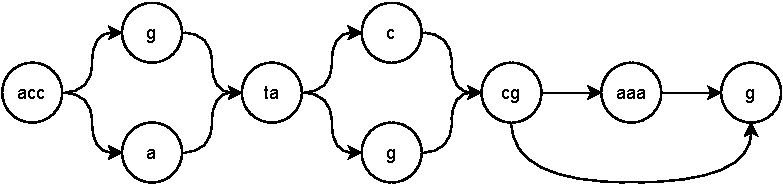
\includegraphics[width=\textwidth]{img/gra.pdf}
  \end{figure}
\end{esempio}
Studiando i cammini dei grafi ottengo tutte le rappresentazioni.\\
Questa rappresentazione però ha dei difetti, in quanto potrei avere cammini che
non rappresentano nessuna sequenza di partenza. Pensando all'esempio sopra
potrei avere il cammino in rosso che non rappresenta nessuna delle tre sequenze:
\begin{figure}[H]
  \centering
  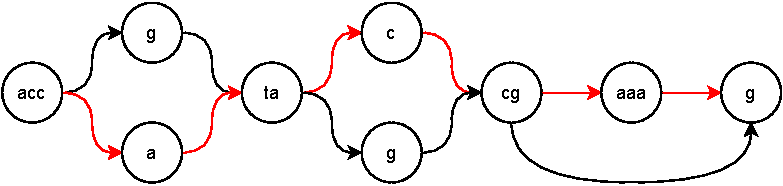
\includegraphics[width=\textwidth]{img/gra2.pdf}
\end{figure}
Rappresento quindi più di quello che voglio rappresentare.\\
Un pangenoma è un grafo che rappresenta una popolazione senza fare grandi
distinzioni, avendo percorsi che non sono riscontrabili in nessun individuo
della popolazione. Si ha comunque che il concetto di sequenza non è più
adeguato. Il grafo di una popolazione è enorme e comunque, tramite colori, si
possono distinguere i vari percorsi della popolazione (distinguendo facilmente
``tracce comuni''). Parlando quindi di \textbf{genoma di riferimento} o si parla
di quello specifico di un individuo o si parla del pangenoma di una popolazione,
con le varianti.\\
Dal punto di vista di \textit{file} le varianti vengono date in un file
\textbf{Variant Call Format (\textit{VCF})}. L'input classico dei software è
quindi spesso un VCF, così come l'output.
\section{Progetti attuali}
Vediamo ora quali sono i grandi progetti su larga scala attualmente in corso:
\begin{itemize}
  \item \textbf{The Cancer Genome Atlas Pan-Cancer Analysis Project
    (\textit{TCGA})}, che cerca di costruire un catalogo delle caratteristiche
  genomiche dei tumori, ovvero un catalogo delle mutazioni genomiche associate a
  tumori (ad esempio quello del seno si sa che è legato alla mutazione del gene
  BRCA che si sa bene dov'è)
  \item \textbf{The 1000 Genomes Project Consortium: A global reference for
    human genetic variation}, che cerca di ricostruire e raffinare un
  sequenziamento di diversi genomi per costruire 
  un genoma di riferimento per una popolazione, nel dettaglio umana, (in formato
  VCF) 
  \item \textbf{Trans-Omics for Precision Medicine}, il progetto per la medicina
  traslazionale 
  \item \textbf{The Computational Pangenome Consortium}, che mira a studiare
  nuovi strumenti software che possano trattare il grafo del pangenoma visto che
  la maggioranza del software attuale ancora funziona su sequenze e non su grafi
\end{itemize}
\section{Sequenziamento del DNA}
Il sequenziamento (che letteralmente significa ``produrre la sequenza'')
solitamente si svolge concatenando diverse operazioni: 
\begin{enumerate}
  \item estrazione del DNA
  \item si ha una ``libreria preparatoria'' dove si mette del materiale genetico
  su un materiale preparatorio
  \item si ha un meccanismo di ``copie'' tramite PCR o simili
  \item si mettono i sample genomici in una macchina di sequenziamento che
  produce in output i dati
\end{enumerate}
Un genoma non può essere letto ``nucleotide per nucleotide'' e i biologi, con la
tecnologia attuale producono le cosiddette \textbf{read} del DNA originali. Si
hanno due tipi di read:
\begin{itemize}
  \item \textbf{read}, dette anche \textbf{short read}, lunghe circa 100
  basi. Illumina produce tendenzialmente 100 o al più 150 basi
  \item \textbf{long read}, lunghe circa 10000 basi (se non di più, anche 20000)
\end{itemize}
Per ottenere il sequenziamento si ha un processo in cui:
\begin{itemize}
  \item si divide il genoma in due parti, ``aprendo'' il filamento di DNA per
  permetterne la lettura
  \item si ha la \textbf{generazione delle read} da copie multiple del genoma
  tramite un processo biologico svolto dai macchinari, che sfruttano processi
  chimici 
  \item si ha poi \textbf{l'assemblaggio dei frammenti}, ovvero un processo
  computazionale dove tramite algoritmi si assemblano le varie read per ottenere
  il genoma di partenza, avendo che le read hanno pezzi in \textit{overlap}
\end{itemize}
Il problema del sequenziamento risale alla fine degli anni settanta con Sander e
Gilbert che avevano studiato un processo di replicazione dando le basi allo
studio del sequenziamento.\\
Dopo il sequenziamento dell'uomo si è passati a sequenziare molti altri
organismi.\\
Oggi il sequenziamento è reso semplice dalla tecnologia. Un esempio è la
tecnologia MinION, così piccola sta stare in una mano, che produce \textit{long
  read} (anche se comunque con diversi errori). MinION è una tecnologia di
\textit{Oxford Nanopore}. MinION è USB ed è fatta per
biologi che devono sequenziare in situazioni d'emergenza (esempio banale un
biologo in Africa in piena emergenza Ebola). L'elaborazione dati viene fatta da
un server.\\
Il primo sequenziamento è costato 3 miliardi di dollari per diversi anni, ora si
fa in meno di 40 ore a 5000 dollari. Di recente si è passati addirittura a poche
ore per un costo di circa 1000 dollari. Tornando alla \textit{legge di Moore} si
ha che il costo è collassato rispetto alla legge e quindi la capacità delle
tecnologie di sequenziamento è molto maggiore della capacità di processare i
dati, per quanto visto ad inizio capitolo. Si hanno quindi tanti dati ma non si
è in grado di elaborarli.\\
Si tratterà anche il \textbf{confronto di genomi} per studiare poi gli aspetti
evoluzionistici, tramite \textbf{alberi evolutivi}, anche \textbf{alberi
  evolutivi tumorali}. Il \textbf{confronto tra sequenze} 
permette di studiare le evoluzioni, anche quelle tumorali, dove si hanno
mutazioni radicali di DNA. Approfondiremo anche tali mutazioni e il loro effetto
(basta il cambio di una base per portare, ad esempio, all'anemia
falciforme). Studieremo quindi anche come fare gli\textbf{
  allineamenti}. Approfondiremo il discorso della \textbf{filogenesi} e della
\textbf{filogenesi tumorale}.\\
Tutto questo, in questo ultimo anno, è stato applicato allo studio di
\textbf{sars-cov-2}, avendo lo studio delle variazioni. \\
Verrà approfondito anche il discorso del \textbf{riarrangiamento}.
\chapter{Grafi di assemblaggio}
La prima tematica che affrontiamo è l'assemblaggio delle read tramite grafi. Per
questo problema abbiamo quindi:
\begin{itemize}
  \item \textbf{input}: collezioni di read (short read e/o long read)
  \item \textbf{output}: grafo di assemblaggio da cui estrarre un cammino o
  un'unica sequenza
\end{itemize}
Si hanno principalmente due tipi di grafo:
\begin{itemize}
  \item \textbf{grafo di De Bruijn (\textit{DBG})} (\textit{si legge ``grafo di
    de broin''}), che si prestano più per \textit{short read} (da 100 o 150
  basi) 
  \item \textbf{grafo di overlap}, più comodo in caso di \textit{long read}
\end{itemize}
Si useranno per questi scopi varie nozioni, tra cui:
\begin{itemize}
  \item relazione di prefisso/suffisso tra k-mers
  \item relazione di prefisso/suffisso tra read
  \item Longest Common Prefix tra sequenze
  \item estrazione di cammino di Eulero dal grafo
  \item estrazione di cammino Hamiltoniano dal grafo
  \item Maximal Exact Matches (\textit{SMEMs})
  \item Burrows Wheeler Transform (\textit{BWT})
  \item indici succinti (come FM-Index)
  \item suffix tree e suffix array
  \item bloom filters, nati in ambito fisico e usati ora in ambito BigData
  \item min-hash e min-sketch, usati anche nelle reti neurali e nel Deep
  Learning quando si ha a che fare con grandi moli di dati
\end{itemize}
Studiare i grafi di assemblaggio può essere utile anche in ottica di applicare
procedimenti simili ad altri problemi posti dai biologi.
\section{Grafi in bioinformatica}
In bioinformatica infatti uno strumento molto usato, anche oltre il
sequenziamento, è quello dei \textbf{grafi}.\\
In letteratura la nozione di grafo compare nel 1735 con il \textbf{grafo di
  Eulero}, con Eulero che, si dice, fosse ossessionato dal problema dei
\textbf{ponti di K\"{o}nigsberg}, volendo trovare il ciclo che attraversasse
ogni ponte solo una volta. Ogni isola di K\"{o}nigsberg diventava un nodo e ogni
ponte tra isole un arco tra nodi. Da qui la definizione del problema.
\begin{definizione}
  Il  \textbf{problema del ciclo Euleriano} consiste nel trovare un ciclo in un
  grafo tale che visiti ogni arco una e una sola volta prima di tornare al punto
  di partenza. Si può passare dallo stesso nodo più volte.\\
  Questo problema si dimostra risolvibile in \textbf{tempo lineare} sull'input
  $G=(V,E)$. 
\end{definizione}
Vediamo poi il ``problema duale'', quello in cui si vuole fare un cilo che non
visiti due volte uno stesso nodo.
\begin{definizione}
  Il  \textbf{problema del ciclo Hamiltoniano} consiste nel trovare un ciclo in
  un grafo tale che visiti ogni vertice una e una sola volta prima di tornare al
  punto di partenza.\\
  Questo problema si dimostra essere \textbf{NP-complete}.
\end{definizione}
La differenza di complessità di questi due problemi sarà qualcosa che bisognerà
considerare parlando dello studio dei grafi in bioinformatica. Anche solo il
problema dell'assemblaggio si vedrà è riducibile alla visita di un grafo (quindi
non potremo formularlo come un problema di ciclo Hamiltoniano, la cui soluzione
potrebbe richiedere anni).\\
La comparsa dei grafi nel mondo chimico è intorno a metà del 1800 con Cayley che
li usò per rappresentare strutture chimiche, nel dettaglio usò \textbf{alberi}
(che ricordiamo esserei grafi connessi aciclici) per contare gli isomeri
strutturali.\\
In biologia l'uso dei grafi è stato introdotto a metà 1900 con l'esperimento di
Benzer, che capì l'importanza dei grafi mentre cercava di distinguere quando
determinati virus attaccano determinati batteri. Benzer è riuscito a mostrare
che il DNA di questi virus era \textit{lineare} mentre prima si congetturava che
il DNA avesse delle biforcazioni. Per capire che non avesse delle biforcazioni
ha sfruttato la capacità di alcuni geni dei virus di aggredire batteri,
rappresentando la cosa coi \textbf{grafi ad intervallo}.
\begin{definizione}
  Nella teoria dei grafi, un \textbf{grafo d'intervallo} è il grafo
  d'intersezione di un 
  multiinsieme di intervalli sulla linea reale. Ha un solo vertice per ciascun
  intervallo dell'insieme, e uno spigolo tra ogni coppia di vertici
  corrispondenti agli intervalli che
  intersecano.\\
  In poche parole associo una lettera ad ogni intervallo e collego nel grafo i
  vertici corrispondenti alla lettera qualora i due intervalli abbiano
  sovrapposizioni.
\end{definizione}
Il punto di svolta si ha però nel 1977 col sequenziamento e i due metodi di
Sanger (che è tutti gli effetti il primo metodo di sequenziamento) e Gilbert,
entrambi chimici. Entrambi i metodi generano frammenti etichettati di lunghezza
variabile che vengono ``letti'' tramite elettroforesi. \\
\textit{Non approfondiamo nel dettaglio i metodi, essendo prettamente chimici e
  biologici}.
\subsection{Superstringhe e grafo di overlap}
Siamo in ottica \textbf{short read sequencing} del \textbf{fragments
  assembly}.\\ 
L'assemblaggio dei frammenti del DNA è invece un problema prettamente
computazionale, avendo l'assemblaggio dei singoli frammenti, ovvero delle
\textbf{read} prodotte dal sequenziamento, anche in più copie, in un'unica
sequenza genomica, detta \textbf{superstringa}. \textit{Fino alla fine degli
  anni '90 l'assemblaggio di frammenti del genoma umano era visto come un
  problema intrattabile.}
\begin{definizione}
  Definiamo \textbf{stringa} come la concatenazione di simboli di un alfabeto
  $\Sigma$.\\
  In bioinformatica spesso si ha $\Sigma=\{a,c,g,t\}$
\end{definizione}
\begin{definizione}
  Definiamo il \textbf{shortest superstring problem (SSP)} come la ricerca,
  dato un insieme di stringhe, di trovare la più corta superstringa che le
  contiene tutte. So hanno quindi:
  \begin{itemize}
    \item \textbf{input}: una collezione $s_1,s_2,\ldots,s_n$ di stringhe che
    possono anche essere lunghe uguali o a lunghezza variabile
    \item \textbf{output}: una stringa $s$ che contiene tutte le stringhe
    $s_1,s_2,\ldots,s_n$ dell'input come sottostringhe tale che $|s|$, ovvero la
    lunghezza della stringa $s$, sia \textbf{minima}
  \end{itemize}
  Questo problema è \textbf{NP-complete} e assume che non ci siano errori di
  sequenziamento nella produzione delle stringhe $s_1,s_2,\ldots,s_n$.\\
  \textbf{La shortest superstring potrebbe non essere unica}.
\end{definizione}
\begin{esempio}
  Vediamo un esempio di shortest superstring. Si assume per semplicità alfabeto
  binario $\Sigma=\{0,1\}$.\\
  Si ha la collezione di stringhe binarie in input (che nel dettaglio sono tutte
  le possibili combinazioni di 3 simboli binari):
  \[C_I=\{000,001,010,011,100,101,110,111\}\]
  Si può verificare che la shortest superstring è:
  \[s=0001110100\]
\end{esempio}
Con la shortest superstring ho letteralmente assemblato le stringhe in input.\\
Le read determinano la \textbf{coverage (\textit{copertura})} del DNA. Per
valutare il coverage vado a vedere ogni base da quante read è coperta. Con
Illumina ho un coverage di almeno 50x, quindi ogni posizione è coperta da almeno
50 read (lunghe ciascuna $\sim$150 basi). Per poter ricostruire la sequenza di
DNA originale serve una certa quantità di coverage. Una coverage bassa potrebbe
impedire la ricostruzione. Illumina va dal 50x minimo anche a 80x.
MinION, della Oxford Nanopore, produce long read anche di 20000 basi ma con
basso coverage, anche 3x, ma avendo read lunghe si riesce comunque ad
assemblare. Quindi se ho long read mi basta un basso coverage mentre se ho short
read mi serve un elevato coverage, avendo un insieme di read molto ``fitto'' e
con poca ``sparsità'', in quanto si avrebbero gap, con zone non coperte. Il
coverage è comunque dato ``per media'' e quindi poter comunque avere buchi.\\
Il punto chiave che mi permette di ricostruire il DNA è la sovrapposizione tra
le varie read. Il DNA inoltre ha ripetizioni e questo costituisce, purtroppo, un
limite all'assemblaggio e in merito studieremo il \textbf{fragment assembly
  problem}, che serve anche in altri contesti, oltre a quello dell'assemblaggio
del DNA. Fin'ora abbiamo anche trascurato anche un altro problema, gli
\textbf{errori di sequenziamento}, dati dal fatto che il processo di sequenziare
non è \textit{ottimo}, ovvero privo di errori, dove con errore si intende che
nel DNA si ha una certa base e nella read prodotta dal sequenziamento se ne ha
un'altra. In fase di assemblaggio questo tipo di errore comporta che non si
riesce a sovrapporre bene le read, non potendo vedere più alcuni
\textbf{overlap} tra coppie read. Si ha quindi \textbf{perdita di informazione
  dell'overlap} e diventa più complicato assemblare il DNA, non impossibile ma
più complicato.
\begin{esempio}
  Si hanno un pezzo di DNA e tre read che sono sovrapponibili:
  \begin{table}[H]
    \centering
    \begin{tabular}{cccccccccc}
      \hline
      & 1 & 2 & 3 & 4 & 5 &6 &7 &8\\
      \hline
      $DNA=$ & a & c & c & g & t &a &c &g\\
      \hline
      $R_1=$ & a & c & c & g & t &&&\\
      $R_2=$ &  & c & c & g & t & a &&\\
      $R_3=$ &  &  &  & g &t & a &c & g&\\
    \end{tabular}
  \end{table}
  Possiamo quindi assemblare il pezzo di DNA.\\
  Ma se ipotizziamo di avere un errore di sequenziamento con la terza base della
  seconda read:
   \begin{table}[H]
    \centering
    \begin{tabular}{cccccccccc}
      \hline
      & 1 & 2 & 3 & 4 & 5 &6 &7 &8\\
      \hline
      $DNA=$ & a & c & c & g & t &a &c &g\\
      \hline
      $R_1=$ & a & c & c & g & t &&&\\
      $R_2=$ &  & c & c & \textbf{c} & t & a &&\\
      $R_3=$ &  &  &  & g &t & a &c & g&\\
    \end{tabular}
  \end{table}
  Diventa più difficile assemblare.
\end{esempio}
Il tasso di errore nei macchinari Illumina è dello 0.01\%, avendo circa due
errori per read lunga 150. Per MinION si ha un tasso d'errore anche di circa il
10\%, quindi ogni 50 basi ho una serie d'errore. Di recente, in ambito long
read, si stanno progettando i \textbf{PacBio HiFi} (con HiFi che qui sta per
``high quality framents'') che producono long read con tasso d'errore allo
0.1\%, facendo ben sperare per il futuro.\\
Tra i primi informatici che hanno fatto sequenziamento abbiamo Eugene Myers che
era un esperto di algoritmi su stringhe e di pattern matching (parte attiva
nella creazione dei suffix array), nonché responsabile della creazione
dell'algoritmo di assemblaggio (famoso anche per BLAST). Eugene Myers era un
esperto del problema della shortest superstring. A partire dalla tecnica di
costruzione della shortest superstring ha sviluppato l'algoritmo di
assemblaggio. Vediamo quindi, in primis, come costruire la shortest
superstring. Per farlo bisogna in primis capire come confrontare le varie
stringhe in input e come ``foldarle''. Per farlo faccio l'overlap che però a
questo punto necessita di una definizione formale.
\begin{definizione}
  Definiamo \textbf{overlap} tra una coppia di stringhe $s_i$ e $s_j$ in input
  come il più lungo prefisso di $s_j$ che ha un match perfetto (coincide) con un
  suffisso di $s_i$. Posso anche dire che è il più lungo suffisso di $s_i$ che
  ha un match perfetto con un prefisso di $s_j$, ribaltare la definizione non
  cambia. L'overlap tra le due stringhe si indica con: 
  \[ov(s_i,s_j)\]
  Ricordiamo che una stringa la posso scrivere in modo scomposto in due modi:
  \begin{itemize}
    \item $s_i=s_i'x$, con $x$ suffisso
    \item $s_j=xs_j'$, con $x$ prefisso
  \end{itemize}
  Tendenzialmente si prende l'\textbf{overlap più lungo}.
\end{definizione}
\begin{esempio}
  Siano:
  \[s_i=accgtgtgt\]
  \[s_j=gtgtgtccaa\]
  Allora si ha che:
  \[ov(s_i,s_j)=gtgtgt\]
  con l'overlap lungo 6.
\end{esempio}
Proseguiamo quindi con il calcolo della shortest superstring dopo aver calcolato
l'overlap di tutte le stringhe in input.\\
Creo un grafo con un nodo per ogni sequenza, etichettato con la sequenza
stessa. Tracciamo quindi un arco tra due nodi sse i due nodi sono in overlap,
associando all'arco la lunghezza dell'overlap.\\
Una tecnica per fare il grafo consiste in:
\begin{itemize}
  \item collegare a priori di tutti i nodi ottenendo un grafo completo non
  orientato 
  \item per ogni coppia di stringhe $s_i$ e $s_j$ metto l'arco pesato con
  l'overlap massimo $ov(s_i,s_j)$, dando anche direzione all'arco. Eventualmente
  posso anche dare doppio peso all'arco in base alla direzione. Si è ottenuto il
  \textbf{grafo di overlap}, che quindi è un grafo orientato (se in entrambi i
  versi non ho overlap lo lascio per praticità senza orientamento con peso 0)
\end{itemize}
\begin{esempio}
  Sia la collezione di stringhe in input:
  \[C_i=\{atc,cca,cag,tcc,agt\}\]
  e costruisco il grafo completo come detto sopra:
  \begin{figure}[H]
    \centering
    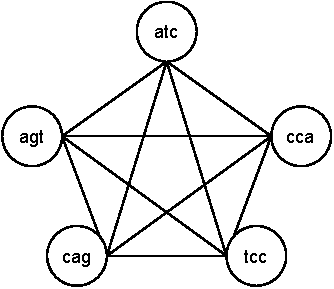
\includegraphics[scale = 0.9]{img/gra3.pdf}
  \end{figure}
  Aggiungo quindi i pesi relativi agli overlap dando l'eventuale orientamento e
  ottengo il grafo di overlap:
  \begin{figure}[H]
    \centering
    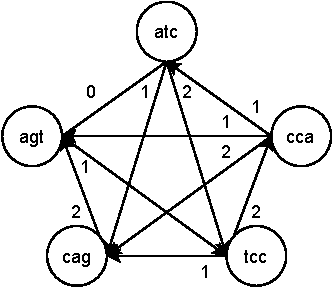
\includegraphics[scale = 0.9]{img/gra4.pdf}
  \end{figure}
\end{esempio}
Per calcolare la shortest superstring dovremo calcolare un certo cammino sul
grafo di overlap. Sicuramente un cammino che visita tutti i nodi mi porta ad
avere una superstringa. Vediamo quindi una prima idea intuitiva:
\begin{esempio}
  Riprendendo il grafo di overlap dell'esempio precedente faccio:
  \begin{itemize}
    \item parto dal nodo $atc$ e lo aggiungo alla superstringa, che per ora è
    $s=atc$ 
    \item seguo l'arco di peso 2 e arrivo in $tcc$
    \item aggiungo $c$ (ovvero la parte non in overlap) alla superstringa, che
    per ora è $s=atcc$ 
    \item seguo l'arco di peso 2 e arrivo in $cca$
    \item aggiungo $a$ (ovvero la parte non in overlap) alla superstringa, che
    per ora è $s=atcca$
    \item seguo l'arco di peso 2 e arrivo in $cag$
    \item aggiungo $g$ (ovvero la parte non in overlap) alla superstringa, che
    per ora è $s=atccag$
    \item seguo l'arco di peso 2 e arrivo in $agt$
    \item aggiungo $t$ (ovvero la parte non in overlap) alla superstringa, che
    per ora è $s=atccagt$ 
    \item mi fermo avendo visitato tutti i nodi
  \end{itemize}
  Alla fine ho:
  \[s=atccagt\]
  che so essere una superstringa.
\end{esempio}
Si vede che il cammino, a conferma, tocca ogni vertice una e una sola volta,
avendo un cammino Hamiltoniano ma, avendo i pesi, abbiamo a che fare con un
\textbf{Traveling Salesman Problem (\textit{TSP})}. Dobbiamo però dimostrare che
la superstringa ottenuta è anche la più breve. \\
Diamo però una piccola definizione formale del grafo di overlap.
\begin{definizione}
  Definiamo il \textbf{grafo di overlap} $G_{ov}=(V,E)$ tale che, data una
  collezione di stringhe $s_1,\ldots,s_n$:
  \begin{itemize}
    \item $V=\{s_1,\ldots,s_n\}$
    \item $E$ è definito in modo che ogni arco $(s_i,s_j)\in E$ è un arco
    orientato da $s_i$ a $s_j$ di peso $|ov(s_i,s_j)|$ (quindi pesato con la
    lunghezza dell'overlap)
  \end{itemize}
\end{definizione}
Si dimostra poi che il \textbf{cammino Hamiltoniano di massimo costo}
``produce'' una shortest superstring. Facciamo una dimostrazione non
formale. Innanzitutto per ``produce'' si intende che, dato il cammino prodotto
da Hamilton di massimo costo, con i vertici etichettati dalle stringhe
$s_{i,1},s_{i,2},\ldots,s_{i,n}$, la superstringa si ottiene sapendo che una
stringa $s_{i,j+1}$ che è ha un prefisso in overlap con al precedente stringa
$s_{i,j}$ la si può scrivere come: 
\[s_{i,j+1}=ov(s_{i,j},s_{i,j+1})\cdot x_{i,j+1}\]
Possiamo anche dire che:
\[r(s_{i,j},s_{i,j+1})=x_{i,j+1}\]
indicando con $x_{i,j+1}$ la parte della stringa fuori dall'overlap, il
``resto'' possiamo dire. A questo
punto so che la superstringa parte con $s_{i,1}$ e prosegue concatenando i vari
$x_{i,j+1}$ (come si può vedere in figura \ref{fig:ssp}):
\[s=s_{i,1}\cdot x_{i,2}\cdot x_{i,3}\cdot\ldots\cdot  x_{i,n}\]

Bisogna dimostrare che il cammino Hamiltoniano di massimo peso coincide con la
shortest superstring. Bisogna dimostrare che:
\begin{itemize}
  \item un cammino Hamiltoniano di massimo peso calcolato come sopra è una
  superstringa, e questo di dimostra perché tocca ogni vertice e quindi ogni
  stringa che di conseguenza viene inclusa
  \item la superstringa appena calcolata è la più breve e per dimostrarlo si ha
  l'intuizione che se massimizzo l'overlap ``globale'' minimizzo la lunghezza
  della superstringa 
\end{itemize}
\begin{figure}
  \centering
  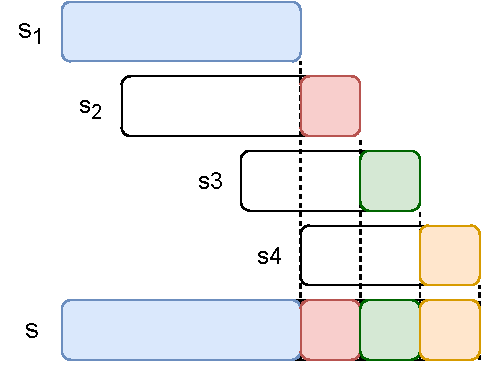
\includegraphics[scale = 0.8]{img/ssp.pdf}
  \caption{Esempio di formazione di una shortest superstring a partire da una
    collezione di stringhe sfruttando i ``resti'' degli overlap}
  \label{fig:ssp}
\end{figure}
Il calcolo della shortest superstring può quindi risolvere l'assemblaggio di
stringhe anche se \textbf{si ricorda che il problema del cammino Hamiltoniano è
  NP-complete}. \\
La miriade di read però, quando ci lavorò per primo Eugene Myers, rendeva
davvero difficile il calcolo (problema NP-complete e hardware storicamente poco
potente). Servirono quindi anni per il primo calcolo, circa una quindicina,
usando appunto il metodo della superstringa.\\
Si ha però un'euristica per calcolare la superstringa, usando un
\textbf{algoritmo 2-approssimante} usando la \textbf{tecnica greedy}. In base a
questa tecnica si sceglie sempre l'arco che pesa di più nel senso che ordino in
ordine di peso tutti gli archi e faccio gli overlap tra le stringhe collegate.
Dopo avere selezionato l'arco si prendono i due estremi e se ne fa la
superstringa. Si continua quindi cercando sempre gli archi che pesano di più
creando poi la superstringa. \textbf{Non si vede nel dettaglio il funzionamento}
e ovviamente non si ha la soluzione ottima e in realtà si congettura sia
2-approssimante ma non si ha una dimostrazione in merito, è un problema aperto
da trent'anni e solo a livello sperimentale si è ipotizzata la
2-approssimazione.\\
Si ricorda che con il cammino Hamiltoniano ottimo si ottiene comunque una
soluzione che potrebbe non essere unica.
\subsection{Grafi di De Bruijn e k-mers}
Siamo sempre in ottica \textbf{short read sequencing} del \textbf{fragments
  assembly}.\\ 
Il metodo della superstringa è stato quindi usato per l'assemblaggio del primo
sequenziamento (quello con il metodo Sanger) ma l'appoggio ad un problema
NP-complete (il \textit{ciclo Hamiltoniano}) rendeva il tutto troppo
dispendioso. Il primo \textit{assemblatore}, quello di Celera, usava però questo
metodo più lento per il \textit{fragment assembly}.\\
Vediamo ora una soluzione diversa, basata sui \textbf{grafi di De Bruijn} che
invece come problema sottostante ha il \textit{ciclo Euleriano} che sappiamo
avere soluzione lineare. \\
Vediamo in primis qualche definizione.
\begin{definizione}
  Definiamo \textbf{k-mer} come è una sottostringa di lunghezza
  $k$. I k-mers sono quindi tutte le sottostringhe distinte di lunghezza $k$,
  non estraggo più volte lo stesso k-mer. Si segnala però che troppe
  ripetizioni dello stesso k-mer, che vengono trascurate, possono rendere
  difficile l'assemblaggio. Quindi il caso ideale è che tutti i k-mer estratti
  da una stringa siano distinti ma si seleziona il $k$ in modo che ci siano al
  più due o tre ripetizioni dello stesso k-mer nella sequenza.
\end{definizione}
\begin{definizione}
  Data una stringa $s$ definiamo \textbf{spettro di $s$ di dimensione/ampiezza
    $l$} è il 
  \textbf{multiinsieme}, \textbf{avendo quindi ripetizioni}, di tutte le
  occorrenze di sottostringhe di lunghezza $l$ (gli l-mers) e si indica con:
  \[spectrum(s,l)\]
  \textbf{Spesso lo spettro poi si rappresenta con i vari l-mer in ordine
    lessicografico}. 
\end{definizione}
\begin{esempio}
  Prendiamo una stringa $s$:
  \[s=tatggtac\]
  Fissiamo $k=3$ e si ha lo spettro di dimensione $3$:
  \[spectrum(s,3)=\{tat, atg, tgg, ggt, gta, tac\}\]
  (\textit{che in questo caso, non avendo ripetizioni, è un insieme di 3-mers.})
\end{esempio}
Dati i frammenti/read (che sono short read lunghe circa 150 basi) si estraggono
da essi i \textbf{k-mers}, con $k$ usualmente pari a 32, 31 o 28 per avere il
minor numero di ripetizioni (i numeri sono stati identificati
sperimentalmente). Si segnala che questa ``proprietà'' di avere sequenze circa
lunghe 32 che non si ripetono è probabilmente legata anche al fatto che il DNA,
preso come sequenza di simboli, è difficile da comprimere con i tool standard
(zip, uso della BWT etc$\ldots$), creando non pochi problemi alle banche dati
anche se ancora non si è scoperto bene ne perché ne come risolvere la cosa.\\  
Il problema di assemblaggio diventa quindi ricostruire una stringa da un insieme
di k-mer:
\begin{itemize}
  \item \textbf{input}: un insieme di stringhe $s_1,s_2,\ldots,s_n$
  \item estraggo i k-mer da tutte le $s_i$ in input, per un $k$ fissato
  \item assemblo i k-mer usando i grafi di De Bruijn
\end{itemize}
Ma prima di introdurre i grafi di De Bruijn vediamo un esempio di cosa
significhi assemblare k-mers, partendo dal caso \textbf{senza ripetizioni},
avendo quindi un \textbf{insieme di k-mers} e non uno \textbf{spettro} (che è un
multiinsieme).
\begin{esempio}
  Si prenda in input una collezione di k-mers con $k=3$ (quindi 3-mers):
  \[C=\{atg, agg, tgc,tcc, gtc, ggt, gca, cag\}\]
  Non essendo coincidenti se facessi gli overlap tra ogni coppia avrei al più
  overlap di lunghezza 2. Ipotizzando di fare il grafo di overlap avrei il
  seguente cammino Hamiltoniano (uno dei possibili):
  \[atg\to tgc\to gca\to cag\to agg\to ggt\to gtc\to tcc\]
  che produrrebbe la superstringa:
  \[s=atgcaggtcc\]
  Vedendo che anche con i k-mer posso ragionare in ottica di superstringa.
\end{esempio}
Ma con l'approccio che vogliamo ora non si passa per ogni vertice una e una
sola volta ma per ogni arco una e una sola volta, usando il cammino
Euleriano.\\
Dobbiamo fare si che quindi prendere ogni arco una e una sola volta
corrisponde a prendere tutti i k-mers, avendo quindi che ogni arco deve essere
associato ad un k-mer. Costruiamo quindi un grafo che soddisfi queste
condizioni (grafo che poi definiremo essere un \textbf{grafo di De
  Bruijn}). Si ha quindi un grafo dove gli archi sono i k-mer mentre i vertici
all'estremo di un arco sono etichettati con il prefisso di lunghezza $k-1$ e
il suffisso di lunghezza $K-1$ del
k-mer (quindi i suffissi e i prefissi unici formano l'insieme dei
vertici). L'arco è orientato dal prefisso al suffisso. \\
In altri termini i vertici agli estremi di un arco etichettato con il k-mer $x$
altro non sono che i due unici (k-1)-mer estraibili da $x$. 
\begin{esempio}
  Prendendo una collezione di k-mer:
  \[C=\{acc,cct,cgt\}\]
  so che, per il grafo $G=(V,E)$, ho $E=C$ mentre per $V$ so che:
  \begin{figure}[H]
    \centering
    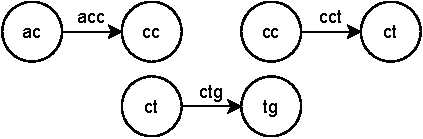
\includegraphics[scale = 1]{img/gra5.pdf}
  \end{figure}
  Quindi $V=\{ac,cc,ct,tg\}$.\\
  Costruiamo quindi il grafo:
  \begin{figure}[H]
    \centering
    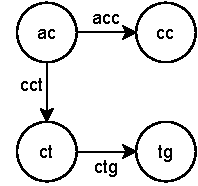
\includegraphics[scale = 1]{img/gra6.pdf}
  \end{figure}
  Quindi il cammino di Eulero (qui banale) e otteniamo la superstringa (e quindi
  l'assemblaggio)
  concatenando le etichette degli archi nell'ordine in cui vengono visitati,
  ragionando nello stesso modo in cui si faceva coi grafi di overlap, quindi
  partendo con la prima etichettata e proseguendo concatenando solo i resti dei
  vari overlap tra etichette degli archi:
  \[s=acctg\]
\end{esempio}
Si ha quindi che:
\begin{definizione}
  Un grafo $G=(V,E)$ \textbf{orientato} è un \textbf{grafo di De Bruijn} di
  ordine $k$ se:
  \begin{itemize}
    \item i vertici sono un sottoinsieme di $\Sigma^{k-1}$, ovvero $V\subseteq
    \Sigma^{k-1}$ 
    \item $\forall u,v\in V$ si ha che $(u,v)\in E$ se esiste una parola $w\in
    \Sigma^*$ tale che $u$ è (ha come etichetta) il prefisso di lunghezza $k-1$
    di $w$ e $v$ è (ha come etichetta) il suffisso di lunghezza $k-1$ di $u$ 
  \end{itemize}
  Quindi possiamo dire che, in modo astratto:
  \begin{itemize}
    \item i vertici sono etichettati con un (k-1)-mer
    \item gli archi sono etichettati con un k-mer
  \end{itemize}
  Tali grafi sono stati introdotti dal matematico De Bruijn nel 1946.\\
  Questa è una definizione \textbf{edge-centric} in quanto i \textbf{k-mer}
  vengono usati per gli archi. Si può avere anche una definizione
  \textbf{node-centric} dove estraggo i nodi per poi ottenere gli archi,
  collegando due vertici quando il prefisso nel primo nodo coincide con il
  suffisso del secondo ma avendo i nodi etichettati coi k-mer. Non
  necessariamente il k-mer dell'arco potrebbe non esistere. Normalmente per
  l'assemblaggio si usa la versione edge-centric. L'edge-centric implica il
  node-centric ma non viceversa. In entrambi i casi etichetto l'arco con il
  resto/estensione. \textbf{Capire meglio!}
\end{definizione}
\begin{definizione}
  Si ha che un vertice è \textbf{bilanciato} sse, $\forall v\in V$:
  \[in(v)=out(v)\]
  con:
  \begin{itemize}
    \item $in(v)$ numero di archi entranti in $v$
    \item $out(v)$ numero di archi uscenti in $v$
  \end{itemize}
\end{definizione}
\begin{teorema}[Teorema di Eulero]
  Un grafo \textbf{connesso} è un \textbf{grafo Euleriano} sse suo ogni vertice
  è \textbf{bilanciato}. 
\end{teorema}
\begin{proof}
  Vediamo le due direzioni della dimostrazione, avendo il \textit{sse}.\\
  Se si ha che per ogni arco entrante nel vertice $v$ deve esistere almeno un
  arco uscente da $v$ in quanto altrimenti mi ``bloccherei'' in un nodo,
  arrivando ad una contraddizione e non avendo quindi un cammino di
  Eulero. Quindi se non è bilanciato sicuramente non è Euleriano.\\
  Se si ha un grafo bilanciato allora esiste (facciamo il caso ``semplice'') un
  ciclo Euleriano (e di conseguenza il caso ``difficile'' del cammino
  Euleriano). Infatti possiamo dare l'algoritmo che trova il ciclo Euleriano. Si
  ha quindi una \textbf{dimostrazione costruttiva}. Si ha quindi che:
  \begin{enumerate}
    \item si parte da un vertice arbitrario $v$
    \item si connette $v$ ad un altro vertice usando archi, si riparte da tale
    arco e si fa la stessa operazione. Si ripete l'operazione fino a che non si
    è formato un ciclo 
    \item alla fine o uso tutti gli archi o altrimenti chiudo un ciclo lasciando
    vertici non usati. Nel secondo caso ripeto lo step 1) cercando di usare
    altri archi non usati. Facendo la \textbf{decomposizione del grafo in
      cicli}. In caso mi fermo quando ho usato tutti gli archi ma mi trovo con
    tanti cicli. Per derivare un unico ciclo da due cicli sfrutto il vertice di
    congiunzione in modo che se entro partendo da un ciclo in quel nodo esco con
    l'arco che mi porta nell'altro ciclo, facendo la cosiddetta \textbf{apertura
      dei cicli} (vedere figura \ref{fig:cic}). \\
    Riassumendo si combinano due cicli in uno unico e si itera questo passaggio
    fino alla creazione di un singolo ciclo. \textit{Per fare questo uso
      l'ipotesi che $G$ è bilanciato}
  \end{enumerate}
  Questo algoritmo è lineare nella dimensione di un grafo, ovvero\\
  $O(|V|+|E|)$.  
\end{proof}
  \begin{figure}
    \centering
    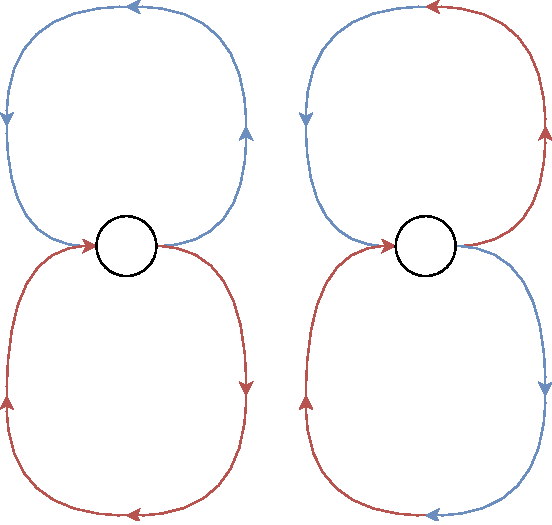
\includegraphics[scale = 0.7]{img/gra11.pdf}
    \caption{Idea del processo di apertura dei cicli dove si hanno due cicli, a
      sinistra in rosso e blu. Dopo l'apertura il cammino passa dal ciclo sopra a
      quello sotto, seguendo i colori nell'immagine a destra.}
    \label{fig:cic}
  \end{figure}
Quindi per costruire il grafo di De Bruijn:
\begin{itemize}
  \item \textbf{input:} una collezione $F$ di frammenti
  \item si genera da $F$ l'insieme dei k-mer (non lo spettro)
  \item per ogni k-mer dell'insieme dei k-mer estraggo il prefisso e il suffisso
  di lunghezza $k-1$
  \item si verifica l'esistenza del cammino di Eulero. Quindi:
  \begin{itemize}
    \item se esiste si prosegue
    \item se non è bilanciato si deve passare alla cosiddetta \textbf{pulitura
      del grafo}, eliminando gli archi detti \textbf{tip} (comportando la
    rimozione anche del nodo ``destinatario'' del grafo). Potrei avere perdita
    di k-mer. Le tip solamente sono singoli archi ma porrebbero anche essere
    cammini.\\
    Si usa anche il concetto di \textbf{bubble}, come effetto degli
    errori di sequenziamento. Una bubble è una situazione in cui si viola il
    teorema di Eulero ma che si elimina essendo un errore di sequenziamento,
    \textbf{risolvendo la bolla}. Per capire quale sia l'errore di
    sequenziamento sfrutto il fatto che ho più read che coprono la stessa
    porzione, scegliendo la base che è più frequente. \textbf{Il $k$ condiziona
      le bolle oltre che alla connettività del grafo (\textit{se è troppo grande
        rischio di non avere un grafo connesso})}.\\
    Spesso si ha anche lo \textbf{scaffolding} per ottenere la connettività
  \end{itemize}
  \item trovo il vertice ``\textit{head}'' (l'unico che non ha vertici entranti)
  e il vertice ``\textit{tail}'' (l'unico che non ha vertici uscenti), che
  saranno inizio e fine del cammino di Eulero
  \item si estrae il cammino di Eulero
\end{itemize}
\begin{esempio}
  Vediamo un esempio di tip, con le tip in rosso:
  \begin{figure}[H]
    \centering
    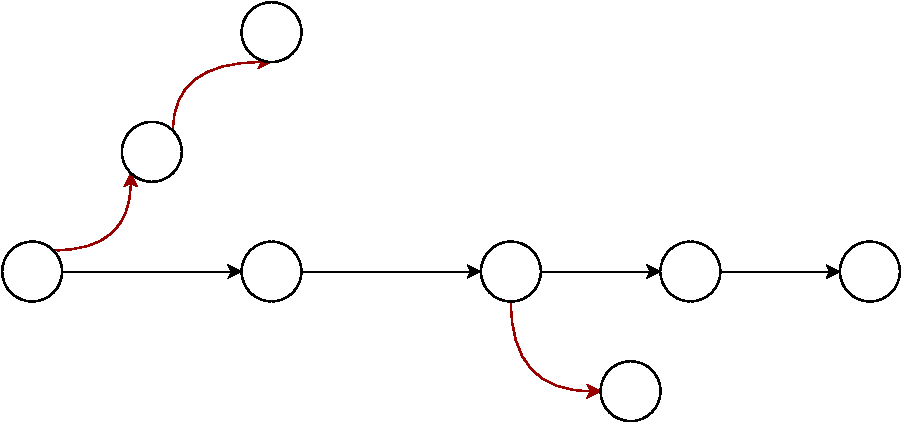
\includegraphics[scale = 0.7]{img/gra9.pdf}
  \end{figure}
  quindi gli archi in rosso e i nodi a cui puntano possono essere rimossi.\\
  Vediamo un esempio di bubble. Ipotizzo di avere:
  \[F=\{acgtatg, acgaatg\}\]
  Notiamo quindi che:
  \[acg\mathbf{t}atg\]
  \[acg\mathbf{a}atg\]
  Ma sappiamo che, tra le varie read, la $t$ occorre molto più frequentemente
  della $a$ in quella posizione.
  Si assuma di avere $k=3$. Ho quindi, con la bolla (notando come la sua
  presenza impedisce di avere un cammino Euleriano) segnalata dall'ovale:
  \begin{figure}[H]
    \centering
    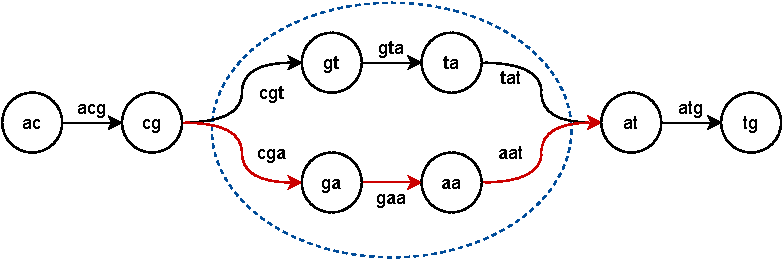
\includegraphics[scale = 0.9]{img/gra10.pdf}
  \end{figure}
  (dove si nota come la $k$ influisca sulla natura della bolla).\\
  Avendo però che la $t$ occorre più frequentemente in quelle posizioni posso
  rimuovere il cammino con gli archi rossi e i due nodi centrali.
\end{esempio}
\begin{esempio}
  Sia:
  \[F=\{atgcc, caatg, gcgtt\}\]
  e sia $k=3$.\\
  Avendo lo spettro:
  \[\{atg, tgc, gcc, caa, aat, atg, gcg, cgt, gtt\}\]
  ho l'insieme dei k-mer, ovvero l'insieme degli archi del grafo,  è:
  \[E=\{atg, tgc, gcc, caa, aat, gcg, cgt, gtt\}\]
  Genero quindi i prefissi e i suffissi di lunghezza $k-1$ di ogni k-mer:
  \[\{at,tg,tg,gc,gc,cc,ca,aa,aa,at,at,tg,gc,cg,cg,gt,gt,tt\}\]
  e quindi l'insieme dei vertici è:
  \[V=\{at,tg,gc,cc,ca,aa,cg,gt,tt\}\]
  Avendo quindi il grafo:
  \begin{figure}[H]
    \centering
    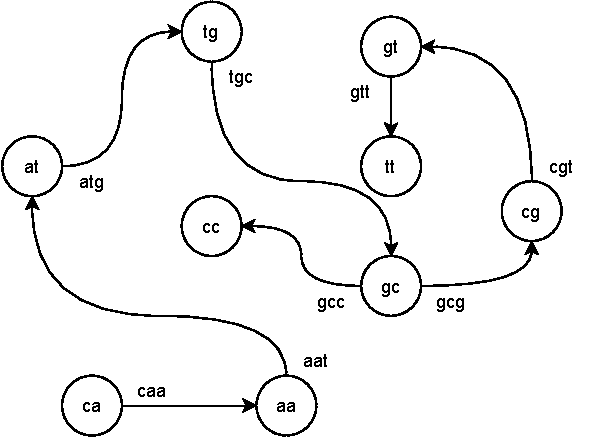
\includegraphics[scale = 1]{img/gra7.pdf}
  \end{figure}
  \textbf{Le etichette degli sono per pura comprensione}.\\
  Bisogna quindi capire se esiste un cammino di Eulero. Purtroppo si hanno i
  vertici con $tt$ e con $cc$ che creano problemi. Inoltre il vertice $gc$ non è
  bilanciato. Quindi il grafo non ammette cammini di Eulero.\\
  Elimino quindi un arco ``problematico'', quello tra $gc$ e $cc$, ottenendo:
  \begin{figure}[H]
    \centering
    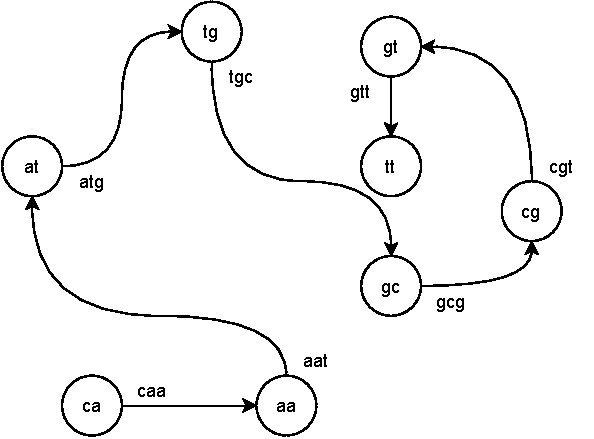
\includegraphics[scale = 1]{img/gra8.pdf}
  \end{figure}
  Dove ho un cammino Euleriano, partendo dal vertice $ca$ e arrivando al vertice
  $tt$. Si compone così la superstringa, ovvero l'assemblaggio: 
  \[s=caatgcgtt\]
\end{esempio}
\begin{definizione}
  Si indica con il termine \textbf{de novo} quando si fa una cosa ``da zero''.\\
  Ad esempio si ha il \textbf{de novo genome assembly}.
\end{definizione}
\begin{definizione}
  Si indica con il termine \textbf{reference bases} quando non si fa una cosa
  ``da zero'' ma si parte da una reference già preesistente. 
\end{definizione}
\section{Note extra sui Grafi}
I grafi di assemblaggio vengono usati anche nella \textbf{metagenomica}, ovvero
lo studio di campioni di DNA di diversi organismi assieme. Questa cosa può
essere utile quando il campione contiene vari organismi, si pensi ad esempio
allo studio di un campione d'acqua o allo studio di un tampone faringeo.\\
\begin{definizione}
  Definiamo il paradigma \textbf{overlap-layout-consesus (\textit{OLC})},
  proposto da Eugene Myers, come il
  paradigma per il quale si procede alla costruzione del grafo a partire da un
  insieme di read. Tramite le read si calcola poi il grafo di overlap per poi
  inferire il cammino, ovvero la \textbf{sequenza di consenso}. Il costo
  computazionale di calcolo non è indifferente.\\
  Rispetto ai grafi di De Bruijn è che possono immediatamente disambiguare brevi
  ripetizioni che i grafici di de Bruijn potrebbero risolvere solo nelle fasi
  successive.
\end{definizione}
\begin{definizione}
  Definiamo formalmente il \textbf{grafo di overlap}.\\
  Dato un insieme di read $R$ un grafo di overlap è un grafo orientato:
  \[G=(R,E)\]
  dove i vertici sono le read stesse e si ha un arco tra $r_i$ e $r_j$ sse un
  suffisso di $r_i$ è un prefisso di $r_j$, essendo in overlap. Il resto
  dell'overlap è detto $e_{ij}$ ed etichetta l'arco (e si nota che il prefisso
  di $r_i$ prima dell'overlap può essere usato come etichetta).
  
\end{definizione}
\begin{figure}
    \centering
    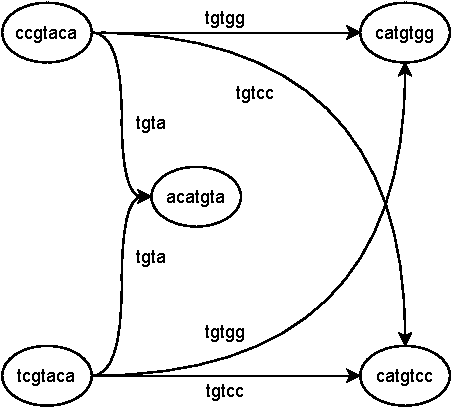
\includegraphics[scale = 0.8]{img/olc.pdf}
    \caption{Esempio di grafo di overlap}
  \end{figure}
Si ha che:
\begin{itemize}
  \item un cammino nel grafo di overlap rappresenta una stringa che è ottenuta
  assemblando le read. Tale stringa è ottenuta tramite $r_1e_{i1}e_{i2}\cdots
  e_{ik}$
  \item se un arco $(r_i,r_j)$ è un cammino con solo due vertici è la stringa
  $s=r_ie_{ij}$ 
  \item  un arco $(r_i,r_j)$ è detto \textbf{riducibile} se esiste un
  percorso da $r_i$ a $r_j$, con anche altri vertici, che rappresenta la stessa
  stringa di $(r_i,r_j)$. Tali archi possono essere eliminati da un grafo di
  overlap ottenendo uno \textbf{string graph}, che offre una struttura più
  semplice e utile per la ricostruzione del genoma
\end{itemize}
Il grafo di overlap può essere usato per trovare le \textbf{varianti}.
\begin{definizione}
  Dato un insieme $R$ di read si ha che un \textbf{edge-centric De Bruijn
    Graph}:
  \[G=(V,E)\]
  di ordine $k$ è un grafo dove i vertici sono i vari (k-1)-mer e si ha un arco
  tra $u$ e $v$ sse esiste un k-mer $w\in R$ tale che si il prefisso di
  lunghezza k-1 di $w$ è uguale a $u$ e il suffisso lungo k-1 di $w$ è
  $v$. L'arco tra $u$ e $v$ è etichettato con l'ultimo carattere di $v$.
  
\end{definizione}
\begin{figure}
  \centering
  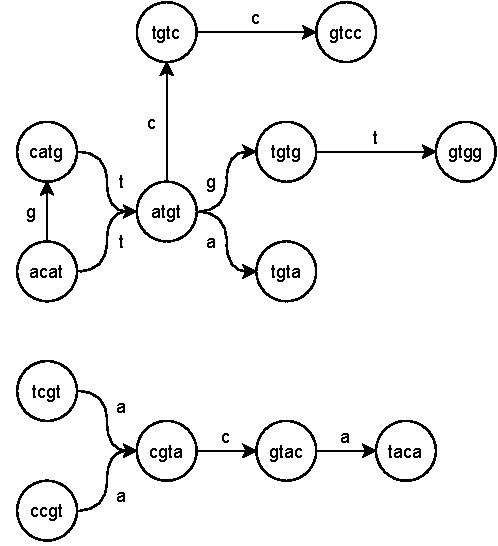
\includegraphics[scale = 0.8]{img/dbg.pdf}
  \caption{Esempio di grafo di De Bruijn con $k=5$ edge-centric (anche se
    rappresentato non con l'intero 5-mer ma solo con il resto).}
\end{figure}
Se teniamo conto che i k-mer sono ripetuti possiamo usare un
\textbf{multigrafo}.
\begin{definizione}
  Un \textbf{multigrafo} è un grafo in cui gli archi sono specificati da un
  \textbf{multinsieme}, il che significa che lo stesso arco può essere ripetuto
  più volte.
\end{definizione}
\begin{definizione}
  Definiamo \textbf{isola} in un grafo di De Bruijn sono un insieme di nodi
  isolati. Sono generate da k-mer non frequenti e quindi probabilmente sono
  errori di sequenziamento.
\end{definizione}
\begin{definizione}
  Definiamo \textbf{tip} in un grafo di De Bruijn come un nodo che si separa
  singolarmente con un arco dagli altri. 
\end{definizione}
I k-mer relativi a isole e tip vanno eliminati.\\
Se si ha che un k-mer è troppo ripetuto si è davanti probabilmente ad una
\textbf{ripetizione}. L'uomo ha molti geni replicati, avendo magari varie
versioni di un certo gene. Posso avere ripetizioni corte o molto lunghe.\\
Oltre alle bolle legate ad errori ho anche bolle legate magari al fatto che
l'uomo è \textbf{diploide}, avendo \textbf{due copie} di ciascun cromosoma, una
ereditata dalla madre e una dal padre, che possono avere comunque il 0.1\% di
differenza. Le read mi arrivano in eguale proporzione dai due cromosomi, sto
assemblando quindi due fonti in una sola sequenza. Nelle banche solitamente si
ha comunque solo l'\textbf{allele di maggioranza} (l'\textbf{allele}, dal punto
di vista informatico, è la base variata a livello di cromosoma). \\
Vanno rimosse anche le \textbf{bubble} e i cammini vengono assemblate nelle
stringhe dette \textbf{contigs}.\\
Un assemblatore che usa i grafi di De Bruijn è davvero complesso.\\
Nell'ultimo periodo in realtà si lavora con una reference e con un file VCF
contenente le varianti. Le read da cui si parte solitamente sono a lunghezza
fissata. \\
In fase di metagenomica si parte da read ``colorate'' provenienti da diversi
organismi. Si costruisce un \textbf{grafo di De Bruijn misto} da cui si riesce
ad estrarre le sequenze delle singole specie. Per farlo si sfruttano varie
informazioni, ad esempio la concertazione di copie di una certa read per le
varie specie. Come informazione si usa anche il fatto che alcune specie hanno
k-mer \textbf{unici}. \\
Diamo uno sguardo anche ai tempi computazionali, con $n$ basi, $g$ lunghezza del
genoma e $a$ lunghezza overlap (con ST indichiamo con \textit{suffix array}, con
DP \textit{programmazione dinamica} e con NE \textit{senza errori}): 
\begin{table}[H]
  \centering
  \begin{tabular}{c|c|c}
    &\textbf{\textit{De brujin}} &\textbf{\textit{Overlap}}\\
    \hline
    tempo & $O(n)$ & $O(n+a)$ ST, $O(n^2)$ DP\\                 
    \hline
    spazio & $O(n)$, $O(\min\{N,g\})$ NE, & $O(n+a)$
  \end{tabular}
\end{table}
Normalmente il sequenziamento viene fatto tramite \textbf{elettroforesi} ma
picchi irregolari portano sicuramente ad errori di sequenziamento.\\
Tornando al discorso \textbf{ripetizioni} si ha che essere conferiscono
``confusione'' all'assemblaggio.\\
\textbf{Risentire ultimi minuti lezione 16 marzo}\\
Potrei avere, con Illumina, buchi di read non coperti che vengono colmati in
modo algoritmico, tramite \textbf{contigs} che si collegano in
\textbf{supercontigs}. Questa operazione è detta \textbf{scaffolding}.
\subsection{Sequenziamento per Ibridazione}
\textbf{Sezione molto oscura.}\\
Per leggere porzioni di DNA si usa il \textbf{sequenziamento per ibridazione
  \textit{SBH}}, ad esempio per leggere le porzioni atta a capire il test di
paternità. Viene fatta tramite \textbf{affymetrix chip}, ovvero una piastra di
materiale plastico dove viene depositato, dentro celle, il DNA da studiare. Il
DNA sfrutta la complementarietà delle basi e queste celle contengono particolari
k-mer così che le celle mi restituiscono i k-mer completi, ottenuti tramite il
processo chimico dell'ibridazione che fa attaccare basi complementari.\\
Si ha quindi il \textbf{SBH problem}, che consiste di ricostruire una stringa
dai suoi l-mer, con:
\begin{itemize}
  \item \textbf{input}: un insieme $S$ con tutti gli l-mer di una stringa $s$
  \item \textbf{output}: una stringa $s$ tale che $Spectrum(s,l)=S$
\end{itemize}
Si usa il cammino Hamiltoniano per risolvere il problema oppure posso usare il
cammino di Eulero usando i (k-1)-mer e il grafi di De Bruijn.

\chapter{Allineamento di Sequenze}
L'\textbf{allineamento} è la procedura principe usata per comparare sequenze
biologiche. \\
Il confronto di sequenze, tramite sequenze di genomi, permette di creare
\textbf{alberi di filogenesi}, alberi no-rooted con le specie attuali come
foglie, che rappresentano l'evoluzione delle varie specie. La ricostruzione di
tale albero avviene grazie al confronto, tramite allineamento, di sequenze.\\
Confrontare le sequenze consiste nello studiare il processo di evoluzione,
risalendo al processo evolutivo tramite le varie mutazioni del DNA.\\
SI hanno due tipi di mutazioni:
\begin{itemize}
  \item a livello nucleotidico, su singole basi, che sono \textbf{operazioni di
    edit}. Una singola base comporta la creazione di una diversa proteina e
  potrebbe portare a varie patologie. Le varie forme di una malattia genetica
  (tipo l'anemia) possono derivare da proteine diverse. A questo tema si
  affianca la medicina traslazionale
  \item a livello più ampio, cromosomico, che riguardano
  \textbf{riarrangiamenti}, ovvero scambi di pezzi di DNA o inversione di
  orientamento di alcune porzioni. Questo è legato magari a fenomeni ambientali
  e comporta il cambiamento di proteine e caratteristiche della specie,
  comportando un processo di adattamento e selezione naturale
\end{itemize}

Con l'allineamento si confrontano sequenze per vedere quanto sono
simili/diversi. Si vuole o massimizzare la simiglianza o minimizzare le
differenze. Per allineare si inseriscono i \textbf{gap}.
% insierire tabella
\begin{table}[H]
  \centering
  \begin{tabular}{c||c|c|c|c|c|c|c|c|c}
    \hline
    \textbf{v}& a& t & & g& t & t& a & t &\\
    \hline
    \textbf{w}& a& t &c & g& t & & a &  &c\\
    \hline
  \end{tabular}
\end{table}
Il biologo attribuisce alle mutazioni un punteggio, uno \textbf{score}. Tale
score è stabilito attraverso uno studio probabilistico sulle mutazione avvenute
nel corso dell'evoluzione.\\
Se allineo più di due sequenze parlo di \textbf{allineamento multiplo}. Si
segnala che il 98\% dei geni è pari tra due mammiferi e si ha più del 70\% di
similarità nelle sequenze proteiche.\\
L'allineamento dal punto di vista algoritmico è fatto tramite programmazione
dinamica (mentre all'inizio erano fatte a mano dai biologi). Dal punto di vista
bioinformatico l'allineamento è il processo base per praticamente qualsiasi
software.
\begin{figure}
  \centering
  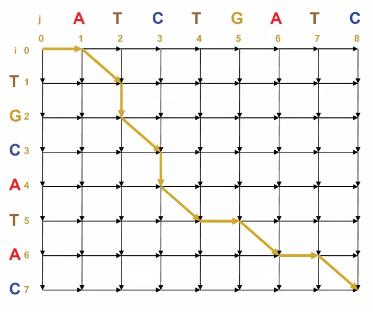
\includegraphics[scale = 0.6]{img/almat.jpg}
  \caption{Esempio di matrice di programmazione dinamica per calcolare
    l'allineamento, dove si hanno 4 match, due inserzioni e due delezioni (si
    ragiona dal punto di vista di $v$).} 
\end{figure}

\begin{definizione}
  Definiamo l'allineamento di due sequenze $A$ e $B$ su $\Sigma^*$ è una matrice
  $A^{2\times l}$ in cui la prima riga è associata ad $A$ e la seconda a
  $B$. Ciascuna riga contiene i caratteri della sequenza associata
  intervallati da gap/spazi, rappresentati con il trattino.\\
  \textbf{Non è permesso avere due gap nelle due righe per la stessa
    posizione. In altri termini non posso avere una colonna di gap}.\\
  Ne segue che al massimo, avendo $|A|=n$ e $|B|=m$ allora:
  \[l\leq n+m\]
  e la matrice $2\times n+m$, ovvero quella massima, consiste nell'avere la
  prima sequenza allineata con soli gap (che saranno sotto) e la seconda
  allineata con soli gap (che saranno sopra).
\end{definizione}
Per definire il problema dell'allineamento ottimo ho bisogno di una:
\[\delta:(\Sigma\cup\{-\})^2\to\mathbb{R}^+\]
Potrei avere anche versioni della delta con pesi negativi:
\[\delta:(\Sigma\cup\{-\})^2\to\mathbb{R}^-\]
dove $\delta$ rappresenta la \textbf{funzione di score}, tramite \textbf{matrice
  di punteggio}, che ha i caratteri 
dell'alfabeto che etichettano righe e colonne. Ogni $a_{ij}$ è lo score.
Sulla diagonale avrò soli 0.\\
Dati in input quindi $A$, $B$ e $\delta$ si ha che il costo della matrice di
allineamento $M$ è il minimo (o a seconda massimo) della somma del costo delle
colonne: 
\[c(M)=\sum_{1\leq i\leq l}\delta(M_{1i,2i})\]
Dove $A_{1i,2i}$ è una scrittura $M[1,i],M[2,i]$.\\
In altri termini è la somma delle delta delle colonne (delta prima colonne più
delta seconda, più delta terza etc$\ldots$).\\
La \textbf{distanza di edit} è un caso particolare dell'allineamento.\\
Il problema \textbf{LCS} (che quindi può essere vista come caso particolare
dell'allineamento), dove date due sequenze $A$ e $B$ si cerca la lunghezza 
della più lunga sottostringa comune, è calcolabile tramite la \textbf{matrice di
  allineamento}, dove l'unico elemento della matrice che costa 1 è quando si ha
un match ($\delta(\sigma,\sigma)=1$), avendo alla fine che che
$c(M)=|lcs(A,B)|$.  \\
Se passo all'\textbf{allineamento multiplo di sequenza} ho in input ho
$A_1,A_2,\ldots,A_k$ con $k$ sequenze. 
\begin{definizione}
  Definiamo l'allineamento multiplo di $A_1,A_2,\ldots,A_k$ è una matrice $M$
  di $k$ righe e $l$ colonne con:
  \[l\leq k\cdot \max\{|A_i|\}\]
  tale che la riga i-esima, $\forall 1\leq i\leq k$, di $M$ contiene la sequenza
  $A_i$ intervallata da gap. Anche qui non si possono avere colonne di soli
  gap. È quindi un'estensione/generalizzazione di quanto detto per due
  sequenze. 
\end{definizione}
\begin{definizione}
  Definiamo anche in questo caso lo scoring, avendo che è identico al caso di
  due colonne. Infatti rappresenta il corso di una operazione tra
  \textbf{coppie} di simboli.
\end{definizione}
\begin{definizione}
  Definiamo il \textbf{costo di una matrice di allineamento multiplo}. Tale
  costo dipende da cosa si vuole evidenziare e si hanno varie definizioni
  alternativa. \\
  La definizione classica è quella della \textbf{sum of pairs}, ma anche le
  alternative, tipo \textbf{consesus}, si basa sul dire che il costo è comunque
  in qualche modo la somma dei costi delle colonne della matrice. Bisogna però
  capire come stabilire tali costi. Per farlo penso ad ogni cella di una colonne
  come nodo di un grafo e costruisco un grafo completo. Il \textbf{sum of pairs}
  è il costo di quel grafo completo. Ogni arco tra coppie $\sigma_1$ e
  $\sigma_2$ (con $\sigma_i$ contenuto della cella i-esima della colonna) è di
  peso pari al $\delta(\sigma_1,\sigma_2)$. Confronto quindi ogni cella della
  colonna con ogni altra, calcolando il delta, e faccio la sommatoria:
  \[c(M)=\sum_{1\leq t,s\leq k} \delta(\sigma_t,\sigma_s)\]
  Nel caso del \textbf{consesus} dovrei vedere solo le differenze rispetto ad
  una sequenza reference, anch'essa in input. Confronto tutte le altre sequenze
  contro questa sequenza reference $A^*$. Avrei quindi come grafo un albero con
  la reference come radice. Alla fine sommo i costi degli archi come per il sum
  of pairs. Tale allineamento è anche detto \textbf{star alignment}.\\
  Questi due sono i due metodi principali ma ci possono anche essere altri
  ``mapping'' tra cui prendere alberi specifici basati sull'evoluzione delle
  specie. Questa tecnica è detta \textbf{tree alignment}, confrontando solo
  coppie di un albero specifico di evoluzione.\\
  A seconda dello scoring poi si procede massimizzando o minimizzando.
\end{definizione}
Bisogna quindi capire come calcolare $M$ tale che il costo di $M$ sia ottimo.\\
Per farlo si applica la programmazione dinamica. Per due sequenze lunghe
rispettivamente $n$ e $m$ il costo sarebbe $O(n\cdot m)$, $O(n^2)$ se lunghe
uguali.\\
Per $k$ sequenze si ha sempre la programmazione dinamica ma il costo è più
elevato. Se le sequenze sono in numero fissato si ha $O(l^k)$ ma se non conosco
il numero di sequenze in input il problema diventa \textbf{NP-hard} anche quando
prendo uno score delta banale che soddisfa la disuguaglianza triangolare su
alfabeto binario. Si hanno quindi diverse euristiche per risolvere il problema e
si basano sempre sull'idea del \textbf{consesus}, con tecniche greedy. Un
esempio di software per farlo è \textbf{MAFFT}.
\begin{esempio}
  Date:
  \begin{itemize}
    \item $A_1=accgtc$
    \item $A_2=ccgcc$
    \item $A_3=accttc$
  \end{itemize}
  Ho una possibile (sarebbero diverse) matrice di allineamento, fatta per
  massimizzare i match:
  \begin{table}[H]
    \centering
    \begin{tabular}{c||c|c|c|c|c|c|c|}
      $A_1$& a&c&c&g&t&c&-\\
      \hline
      $A_2$& -&c &c & g&-& c&c\\
      \hline
      $A_3$&a&c&c&t&t&c&-
    \end{tabular}
  \end{table}
  Per esempio per la prima colonne avrei:
  \begin{itemize}
    \item $\delta(a,-)$
    \item $\delta(a,a)$
    \item $\delta(-,a)$
  \end{itemize}
  coi tre valori che andrebbero sommati nel caso di sum of pairs.
\end{esempio}
Fondamentalmente allineare sequenze significa trovare un cammino in una griglia,
un problema del tipo \textbf{Manhattan Tourist Problem (MTP)}. La griglia
rappresenta diversi modi per attraversare la città da un punto $A$ ad uno $B$
dove si hanno pesi per ogni arco (i lati dei quadrati della gruglia hanno un
peso associato) per specificare il numero di attrazioni. Lo
scopo è arrivare alla fine massimizzando il numero di attrazioni viste.\\
Si cerca quindi il cammino più pesante in una griglia pesata. In input si ha la
griglia, il punto di partenza e di arrivo. Una strategia greedy per la quale ad
ogni istante scelgo l'arco più pesante non sempre porta alla soluzione ottima.\\
Si ha quindi un algoritmico di programmazione dinamica con il criterio di
memorizzazione. \\
L'algoritmo ricorsivo si preoccupa di capire come arrivare al nodo finale
ragionando a partire dal nodo finale stesso, sapendo che posso fare solo certi
movimenti sulla griglia. Derivo il costo ottimo di un nodo a partire dai costi
ottimi dei nodi che portano a quel nodo (scegliendo il migliore).
\begin{algorithm}
  \begin{algorithmic}
    \If{$n=0\lor m=0$}
    \State \textbf{return} $MT(n,m)$
    \EndIf
    \State $x\gets MT(n-1,m) + w(u,v),\,\,\, u=(n-1,m),v=(n,m)$
    \State $y\gets MT(n,m-1) + w(z,v),\,\,\, u=(n,m-1),v=(n,m)$
    \State \textbf{return} $\max\{x,y\}$
  \end{algorithmic}
  \caption{Algoritmo MTP con ricorsione}
\end{algorithm}
Con la programmazione dinamica parto dalla sorgente e accumulo il punteggio per
ogni percorso possibile, scegliendo poi il miglior percorso. Visito l'intera
griglia e calcolo ogni volta il modo migliore per arrivare ad un nodo,
risolvendo ogni volta problemi di massimo. Alla fine vado a ritroso per capire
che percorso fare mentre nell'ultimo nodo potrò già vedere il peso ottimo del
percorso scelto.

\[s_{i,j}=\max\
  \begin{cases}
    s_{i-1,j} + w(u,v),\,\,\, u=(i-1,j),v=(i,j)\\
    s_{i,j-1} + w(z,v),\,\,\, z=(i,j-1),v=(i,j)
  \end{cases}
\]
Si a quindi, per una griglia $n\times m$, un costo pari a $O(n\cdot m)$.

Potrei aggiungere al problema l'uso delle diagonali, dovendo cambiare il
sistema, aggiungendo il costo della diagonale:
\[s_{i,j}=\max\
  \begin{cases}
    s_{i-1,j} + w(u,v),\,\,\, u=(i-1,j),v=(i,j)\\
    s_{i,j-1} + w(z,v),\,\,\, z=(i,j-1),v=(i,j)\\
    s_{i-1,j-1} + w(o,v),\,\,\, o=(i-1,j-1),v=(i,j)
  \end{cases}
\]
Trovare un cammino ottimo (uno di quelli più pesanti) della griglia corrisponde
all'allineamento tra sequenze. \\
Dato il costo quadratico di confrontare due sequenze si passa a considerare
anche metodi di confronto \textbf{alignment-free}, dove si decide che due
sequenze sono molto simili senza fare l'allineamento.\\
Per allineare nel modo più veloce possibile si è passati poi dalla
programmazione dinamica i metodi \textbf{bwt-based}.\\
\textit{L'allineamento può essere usato sui k-mer per eliminare a priori errori
  prima della costruzione del grafo di De Bruijn.}\\
\begin{definizione}
  Definiamo il seguente \textbf{paradigma}. La somiglianza/similarità a livello
  di sequenza implica ``stessa funzione''.\\
  Due regioni genomiche, che si sa essere geni, uguali in due specie si ha che
  rappresentano lo stesso gene (e questo permette di studiare i topi in ambito
  medico e farmacologico).\\
  Si rileva che la stessa funzione non implica per forza stessa sequenza e
  quindi stesso gene. Non vale quindi il viceversa.
\end{definizione}
Ricordiamo che il problema MTP consisteva nel trovare il cammino che
massimizzava il cammino in una grigia. La risoluzione usa appunto la
programmazione dinamica.\\
Interpretiamo il riempimento della griglia in termini di confronto di
sequenze.\\
Un allineamento senza mismatch altro non è che il calcolo della Longest Common
Subsequence LCS.\\
Per trovare l'LCS posso usare un grafo pesato che parte da un \textit{source} e
arriva ad un \textit{sink}, trovando all'interno il cammino più pesante dal
source al sink. Ogni cammino è tra il source e il sink. I nodi rappresentano i
confronti tra due simboli delle due 
stringhe di partenza. Se ho un arco diagonale mi sto spostando su entrambe le
sequenze, che in quel nodo hanno lo stesso simbolo. Con gli archi verticali e
orizzontali mi sposto solo in una delle due sequenze, confrontando un simbolo
con un gap (se l'arco è verticale ho un gap nella stringa che sta sulle colonne
e viceversa se ho un arco orizzontale). Il percorso migliore è quello con più
diagonali possibili visto che rappresentano un match. La diagonale ha quindi
costo $\delta(\sigma,\sigma)$, mentre le altre due mosse hanno costo
$\delta(-,\sigma)$ e $\delta(\sigma,-)$. Una matrice di
allineamento è quindi un percorso nella griglia.\\
Ogni volta che ci si allontana dalla diagonale principale si sta inserendo un
gap. Potrei quindi ragionare \textbf{allineando per banda}, avendo al più $k$
gap e quindi costruendo solo una banda distante al più $k$ dalla diagonale
principale, avendo quindi un algoritmo più veloce per costruire
l'allineamento. \\
Si nota quindi che LCS è un MTP e anche la distanza di edit è calcolabile con la
griglia. \\
Per LCS, per due stringhe $v$ e $w$, si ha infatti che:
\[s_{i,j}=\max
  \begin{cases}
    s_{i-1,j}\\
    s_{i,j-1}\\
    s_{i-1,j-1}+1\mbox{ se } v_i=w_j
  \end{cases}
\]
Quindi nella griglia le diagonali costano 1 e gli altri costano 0. \\
Quando si fa l'allineamento si sta calcolando in realtà la \textbf{distanza} tra
due sequenze, calcolando quanto sono diverse. La distanza di edit è una di
queste distanze, che rappresenta il minimo numero di operazioni epr trasformare
una stringa in un'altra. Un altra è la \textbf{distanza di Hamming}, che si
riferisce a sequenze di distanza uguale, senza ammettere spazi, calcolando il
numero di posizioni in cui si hanno mismatch. Non si hanno inserzioni e
delezioni in Hamming, mentre si hanno entrambe in edit.





\chapter{I dati in Bioinformatica}
Dobbiamo introdurre i dati fondamentali della bioinformatica, ovvero
\textbf{DNA} (figura \ref{fig:dna}) e \textbf{RNA}, intese come molecole
biologiche che vengono trattate come stringhe.\\
Il \textbf{DNA (\textit{acido deossiribonucleico})} è una molecola composta da
nucleotidi, che è formato da:
\begin{itemize}
  \item il deossiribosio, uno zucchero, \textbf{D}
  \item un gruppo fosfato, \textbf{p}
  \item una base azotata (Adenina, Citosina, Guanina, Timina). Citosina e Timina
  sono dette \textbf{piramidine}, le altre due \textbf{purine}
\end{itemize}
\begin{figure}
  \centering
  \includesvg[scale = 0.8]{img/dna.svg}
  \caption{Rappresentazione grafica del
    DNA tratta da \url{https://it.wikipedia.org/wiki/DNA}} 
  \label{fig:dna}
\end{figure}
Si ha la cosiddetta \textbf{direzione 5'3'} per leggere le sequenze del DNA
(avendo la direzione posso leggere in sequenza le basi, solitamente è dal basso
all'alto).\\
I nucleotidi si legano tramite \textbf{legame fosfodiesterico tra D e P}. \\
L'unità di lunghezza di un molecola di DNA è il \textbf{base pair
  (\textit{bp})} (base pair in quanto il DNA è in se un'accoppiamento di basi a
doppia elica), ovvero il numero delle basi.\\
Il \textbf{genoma} è la lunga molecola di DNA contenuta in ogni nucleo
cellulare. Nel 1953 Watson e Crick hanno scoperto essere a doppia elica. Il
genoma è frammentato in \textbf{cromosomi} (22 autosomi e i due cromosomi X e
Y). Il più lungo cromosoma è il primo e il più corto è il ventiduesimo.\\
Tra le due catene di un genoma si ha che la Timina si appaia all'Adenina (e
viceversa) mentre la Citosina alla Guanina (e viceversa), questa è la
\textbf{regola delle basi complementari}. Se una catena ha la
direzione 5'3' dall'alto verso il basso l'altra lo ha dal basso all'alto (ma
sempre da 5' a 3') e viceversa. Si legge sempre in direzione 5'3' e si hanno
così le \textbf{due sequenze primarie appaiate}, una detta \textbf{forward
  strand (+,1,+1)} e una detta \textbf{reverse strand (-,-1)}.\\
Tra Adenina e Timina abbiamo due legami idrogeno mentre tra Citosina e Guanina
se ne hanno tre (si richiede quindi più energia per eventualmente separare).\\
Si ha quindi a che fare con un alfabeto $\Sigma=\{a,c,g,t\}$ o
$\Sigma=\{A,C,G,T\}$ per costruire le sequenze. Data la sequenza primaria di una
delle due catene del DNA genomico, la sequenza primaria della catena appaiata è
ottenuta per mezzo di un'\textbf{operazione di reverse\&complement}, ottenuta
sostituendo alla catena primaria ribaltata ogni base con la complementare
(potrei anche prima sostituire e poi invertire). Se
prendo entrambe le stringhe le chiamo \textbf{paired strands}.\\
Aggiungiamo altre definizioni:
\begin{itemize}
  \item una regione di DNA genomico che ha una certa funzione prende il nome di
  \textbf{locus}
  \item la sequenza primaria di un locus è chiamata \textbf{sequenza genomica},
  che di fatto è una sottostringa del genoma di un organismo
\end{itemize}
Per l'\textbf{RNA (\textit{acido ribonucleico})} si ha una composizione di
nucleotidi del tipo:
\begin{itemize}
  \item il ribosio, uno zucchero, \textbf{D}
  \item un gruppo fosfato, \textbf{p}
  \item una base azotata (Adenina, Citosina, Guanina, Uracile)
\end{itemize}
Anche per l'RNA si ha la \textbf{direzione 5'3'} e si ha un alfabeto
$\Sigma=\{a,c,g,u\}$ o $\Sigma=\{A,C,G,U\}$. La vera differenza è che l'RNA è
sempre in \textbf{singola catena}.\\
Una \textbf{proteina} p una catena di amminoacidi e la sua sequenza primaria è
una stringa costruita su un alfabeto di 20 simboli che rappresentano i 20
\textbf{amminoacidi} presenti in natura.
\begin{table}
  \centering
  \begin{tabular}{|c|c|c|}
    \hline simbolo&sigla & nome \\
    \hline A & Ala & Alanina \\
    \hline C & Cys & Cisteina \\
    \hline D & Asp & Acido aspartico \\
    \hline E & Glu & Acido glutammico \\
    \hline F & Phe & Fenilalanina \\
    \hline G & Gly & Glicina \\
    \hline H & His & Istidina \\
    \hline I & Ile & Isoleucina \\
    \hline K & Lys & Lisina \\
    \hline L & Leu & Leucina \\
    \hline
  \end{tabular}
  \begin{tabular}{|c|c|c|}
    \hline simbolo&sigla & nome \\
    
    \hline M & Met & Metionina \\
    \hline N & Asn & Asparagina  \\
    \hline P & Pro & Prolina  \\
    \hline Q & GIn & Glutammina \\
    \hline R & Arg & Arginina  \\
    \hline S & Ser & Serina  \\
    \hline T & Thr & Treonina\\
    \hline V & Val & Valina  \\
    \hline W & Trp & Triptofano \\
    \hline Y & Tyr & Tirosina \\
    \hline
  \end{tabular}
  \caption{Tabella con l'elenco degli amminoacidi}
  \label{tab:ammi}
\end{table}
I \textbf{geni} è il ``responsabili'' della produzione di proteine, che poi
``regolano'' la vita. Ogni proteina è prodotta da un gene e un gene genera più
proteine.\textbf{ I geni sono il 10\% del genoma}, quindi solo una piccola
parte. Il gene è quindi un locus del genoma che esprime una proteina. La
sequenza primaria del locus di un gene è la sequenza genomica del gene. Ogni
gene ha un identificativo detto \textbf{HUGO NAME}, con una precisa nomenclatura
che è ``circa'' un acronimo. Un gene può appartenere al genoma di diversi
organismi. \\
Sia il forward strand che il reverse strand contengono geni e gli uni non
c'entrano con gli altri (figura \ref{fig:gene}). L'uomo ha circa 20000 geni
codificanti (più i cosiddetti \textbf{geni non codificanti} che hanno altri
scopi), ciascuno che  
codifica una o più proteine. Ogni cellula contiene l'intero set di geni che
regolano la vita dell'organismo, ma nelle varie cellule si \textbf{esprime} solo
un sotto-set di geni mentre gli altri rimangono \textbf{inattivi}, è il
\textbf{profilo di espressione}. Può variare anche la quantità di proteina
espressa. In due cellule posso esprimere lo stesso gene che però porta a diverse
proteine. \\
Si ha quindi:
\begin{enumerate}
  \item il locus viene trascritto (con anche lo splicing) nell'm-RNA detto
  trascritto
  \item il trascritto porta alla proteina
\end{enumerate}
  \begin{figure}
    \centering
    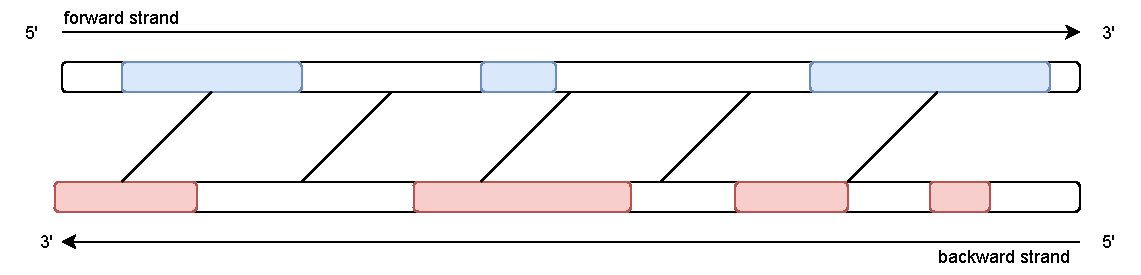
\includegraphics[width=\textwidth]{img/gene.pdf}
    \caption{Rappresentazione stilizzata dei due strand con in azzurro e rosso,
      rispettivamente, i geni sul forward strand e sul backward strand}
    \label{fig:gene}
  \end{figure}
Per determinare la sequenza primaria di DNA e RNA usiamo il sequenziamento,
producendo varie read e procedendo poi alla ricostruzione
\textbf{in-silico}. Posso avere due tipi di output dal sequenziamento:
\begin{itemize}
  \item \textbf{single-end reads}, che è un'unica sequenza
  \item \textbf{paired-end reads} e \textbf{mate-pair reads}, dove si parla di
  coppie di sequenze che sappiamo circa quanto distavano sulla sequenza
  originale 
\end{itemize}
Per il sequenziamento ci sono stati vari step:
\begin{itemize}
  \item \textbf{first generation}, per il \textbf{metodo Sanger} nel 1975. Si
  hanno:
  \begin{itemize}
    \item {\color{OliveGreen}read lunghe fino a 1000bp}
    \item {\color{OliveGreen}elevata qualità}
    \item {\color{Maroon}bassa coverage}
    \item {\color{Maroon}costi elevati}
  \end{itemize}
  \item \textbf{second generation}, con le \textbf{Next-Generation-Sequencing
    (\textit{NGS}) technologies}, dagli inizi degli anni 2000. Si
  hanno:
  \begin{itemize}
    \item {\color{Maroon}read corte, da 100bp a 400bp}
    \item {\color{OliveGreen}alta coverage}
    \item {\color{OliveGreen}bassi costi}
  \end{itemize}
  Tra le tecnologie \textit{NGS} abbiamo:
  \begin{itemize}
    \item Illumina (Solexa) con:
    \begin{itemize}
      \item HiSeq System 
      \item Genome analyzer lix
      \item \textbf{MySeq}, che produce read di 300bp, con il 99.90\% di
      accuratezza, producendo 25 milioni di read per run
    \end{itemize}
    \item Ion Torrent-Life technologies con:
    \begin{itemize}
      \item \textbf{Personal Genome Machine (\textit{PGM})}, che produce read di
      200bp, con il 99.00\% di accuratezza, producendo 11 milioni di read per
      run  
      \item Proton 
    \end{itemize}
  \end{itemize}
  Per indicare i dati prodotti diciamo \textbf{NGS data}
  \item \textbf{third generation}, con le \textbf{Next
    Next-Generation-Sequencing technologies}, più avanti negli anni 2000. Si
  hanno:
  \begin{itemize}
    \item {\color{OliveGreen}read lunghe fino a 10000bp}
    \item {\color{OliveGreen}qualità relativamente bassa}
  \end{itemize}
  Tra le tecnologie \textit{Next-Next} abbiamo:
  \begin{itemize}
    \item Pacific Biosciences con PacBio RS
    \item Oxford Nanopore Technologies con:
    \begin{itemize}
      \item GridION System 
      \item MinION
    \end{itemize}
  \end{itemize}
\end{itemize}
\section{Formato FASTA}
Vediamo il formato standard per sequenze primarie nucleotidiche:
\begin{itemize}
  \item \textbf{FASTA} per le sequenze ottenute al metodo Sanger, quindi con
  pochi errori 
  \item \textbf{FASTQ} per le sequenze ottenute con NGS. È un'evoluzione del
  FASTA in cui si associa alle sequenze dei reads un valore di qualità, uno per
  base 
\end{itemize}
Il FASTA ha le seguenti caratteristiche:
\begin{itemize}
  \item è un plain text
  \item ha la sequenza primaria (ma anche sequenze di amminoacidi) più
  eventuali informazioni extra a scelta. Si ha:
  \begin{itemize}
    \item un header introdotto da $>$ con tutte le informazioni extra in una
    sola riga (tra cui, volendo, cromosoma di partenza, indici di inizio e fine
    per specificare la porzione, ricordando che le posizioni sono 1-based, la
    ``release'', ad esempio tramite la sigla \textit{GRC}, lo strand tramite +1
    e -1 etc$\ldots$)  
    \item la sequenza genomica separata in righe di 60 o 80 bp (quindi dopo 60 o
    80 simboli vado a capo)
  \end{itemize}
  \item è stato pensato come formato di input del software FASTA per
  l'allineamento
  \item ha come estensione \texttt{.fa} o \texttt{.fasta}
\end{itemize}
\subsection{ENSEMBL}
ENSEMBL è il \textbf{genome browser} attualmente più usato. Un genome browser è
un database con associata un'interfaccia di esplorazione. È un progetto partito
nel 1999 da \textbf{EMBL (\textit{European Molecular Biology Laboratory})} e dal
\textbf{Wellcome Trust Sanger Center}. Dal 2017 fa capo a 
\textbf{EMBL-EBI (\textit{European Bioinformatics Institute})}, sempre di
\textbf{EMBL}. Si hanno i dati di 250 specie di cordati, tra cui uomo, topo,
ratto e 
zebrafish. Si hanno vari livelli di informazione (ovvero di annotazioni), tra
cui; genoma, gene, proteina etc$\ldots$\\
I genome browser sono consistenti rispetto a progetti di ricerca e
analisi genomiche. SI può accedere, tra le altre cose a:
\begin{itemize}
  \item la sequenza del genoma di una data specie o dei singoli cromosomi
  \item le sequenze dei geni annotati su di un genoma e i relativi trascritti
  espressi
  \item le variazioni annotate rispetto al genoma di riferimento che
  caratterizzano i singoli individui  
\end{itemize}
\textbf{Le coordinate sono sempre rispetto alla catena forward}.\\
ENSEMBL si può raggiungere tramite \url{www.ensembl.org}.\\
Si ha anche il formato \textbf{EMBL} stesso, pensato originariamente per
memorizzare sequenze 
nucleotidiche in banche dati che non erano db relazionali ed erano senza
accesso. Il file poteva essere scaricato tramite un ID e basta (era poi scopo
del biologo e dell'informatico riutilizzarlo). Il file EMBL è pieno di
informazioni, con in fondo la sequenza nucleotidica. Banche dati così ci sono
ancora, come l'\textbf{ENA (\textit{European Necleotide Archive})}.
\section{Qualità dei Dati e FASTQ}
Valutiamo quindi la \textbf{qualità del dato di sequenziamento} e il formato
standard \textbf{FASTQ}, il formato di output dei sequenziatori di nuova
generazione. \\ 
Le NGS producono una gran quantità di frammenti, piuttosto corti, per i quali è
essenziale conoscere la qualità di ogni base in fase di processamento della
read, per eliminare/modificare le parti problematiche. Per ogni base di una read
NGS si ha quindi un \textit{indice di qualità}, detto \textbf{Phred Quality
  Score}.\\
Phred, abbreviato, è stato creato per il \textit{base caller Phred}, che sfrutta
il cromatogramma che valutare la qualità.
\begin{definizione}
  Definiamo \textbf{Phred Quality Score} $q$ tramite la formula:
  \[q=-10\log_{10}p\]
  con:
  \begin{itemize}
    \item base $b$
    \item $p$ probabilità che $b$ sia errata
  \end{itemize}
  il valore $q$ viene arrotondato all'intero più vicino.\\
  Chiedere una base corretta al 100\% comporterebbe $q=\infty$ (avendo $p=0$) e
  quindi si considera corretta una base con $q\geq 50$ (che comporterebbe
  probabilità che sia errata pari a $p=0.00001$, quindi 0.001\%).\\
  Una base con $30\leq q\leq 50$ è solitamente considerata buona ma dipende dal
  contesto. Avere $q=30$ hanno probabilità delle 0.1\% di essere errate. 
\end{definizione}
\textbf{Esempi su slide}.\\
Il formato \textbf{FASTQ} è standard per i sequenziatori NGS, che quindi non
producono un \textbf{FASTA}.\\
SI ha che è:
\begin{itemize}
  \item plain text
  \item è stato sviluppato per associare ad una sequenza il Phred Quality Score
  \item ha estensione \texttt{.fq} o \texttt{,fastq}
\end{itemize}
Si hanno 4 righe, dette record:
\begin{itemize}
  \item un header con l'identificatore. Tale riga ha ``@'' come simbolo
  iniziale. Non si hanno informazioni extra come per il FASTA
  \item sequenza delle basi della read in una riga
  \item un header dei phred values. Tale riga inizia con il simbolo ``+''
  \item la sequenza dei valori di qualità, una per ogni base della read
\end{itemize}
\begin{esempio}
  Vediamo un esempio:
\begin{verbatim}
@HWUSI-EAS522:8:5:662:692#0/1
TATGGAGGCCCAACTTCTTGTATTCACAGGTTCTGC
+HWUSI-EAS522:8:5:662:692#0/1
aaaa`aa`aa`]__`aa`_U[_a`^\\UTWZ`X^QX
\end{verbatim}
  con:
  \begin{itemize}
    \item l'header della sequenza un identificatore tipico di illumina
    \item le basi su una riga
    \item l'header, con lo stesso identificatore della sequenza (è opzionale,
    potrei non averlo), dei phred
    \item la sequenza dei phred values, con una codifica che permette di
    associare facilmente il valore di qualità. Ogni valore è in corrispondenza
    di indice con la base di cui rappresenta la qualità (se usassi gli interi
    avrei magari un intero di due simboli che renderebbe impossibile capire a
    che base si riferisce)
  \end{itemize}
\end{esempio}
I valori interi di qualità vengono quindi convertiti in un certo carattere e
ogni sequenziatore ha la sua funzione per convertire l'intero rappresentante la
qualità $q$ in char:
\[c=f(q)\]
Ad esempio per Illumina è (con $ASCII(X)$ che converte in char l'intero):
\[c=ASCII(\min\{q,93\}+33)\]
\textbf{Esempi su slide}.\\
Conoscere la qualità delle basi permette di fare \textbf{trimming} che, fissata
una soglia minima di qualità (decisa di volta in volta), consiste in:
\begin{itemize}
  \item trovare la più lunga sottostringa della read composta da basi con
  qualità superiore a questa soglia minima
  \item sostituire tale sottostringa all'intero read sse questa sottostringa è
  lunga a sufficienza (lunghezza anch'essa decisa di volta in volta). Qualora la
  sottostringa sia troppo corta si elimina la read. Su milioni di read
  sacrificarne qualcuna non è un problema particolare e non solo, si migliorano
  le analisi successive
\end{itemize}
\section{Espressione di un Gene e GTF}
Ricordiamo che un gene è un locus che codifica una proteina. La sequenza
primaria del locus di DNA del gene è detta \textbf{sequenza genomica del gene}
(e si ricorda che entrambi gli strand contengono geni, negli esempi si studia
comunque il forward essendo già da ``sinistra a destra'').\\
I geni si identificano tramite il cosiddetto \textbf{HUGO NAME}.\\
I geni sono formati da \textbf{esoni}, regioni codificanti, e
\textbf{introni}, regioni non codificanti. Il confine tra un esone a sinistra
e un introne a destra è detto \textbf{sito di slicing al 5'}, detto anche
\textbf{donor splice site}. Se ho un introne
a sinistra e un esone a destra ho un \textbf{sito di slicing al 3'}, detto
anche \textbf{acceptor splice site}. Nell'uomo il 99.24\% degli introni
iniziano con GT e finiscono con AG e si parla di \textbf{introne canonico}. Si
hanno anche introni non canonici.\\
Vediamo gli step di sintesi proteica in modo ``operativo'':
\begin{itemize}
  \item si ha la \textbf{trascrizione} dove l'intero locus del gene viene
  copiato in una molecola di RNA (convertendo T in U), detta \textbf{pre-mRNA},
  lunga quanto il locus del gene
  \item avviene quindi lo \textbf{splicing}, dove si eliminano gli intorni dal
  pre-mRNA producendo l'\textbf{mRNA}, che è una sequenza continua di esoni, di
  regioni codificanti, detta anche \textbf{trascritto}
  \item il trascritto viene tradotto in proteina. In realtà all'interno del
  trascritto si ha una parte centrale detta \textbf{coding sequence
    (\textit{CDS})} che è la parte che da origine alla traduzione in
  proteina. La CDS inizia sempre con la \textbf{tripletta di inizio} AUG e
  finisce con una tra le seguenti \textbf{triplette di fine} UAG, UAA o UGA. La
  lunghezza della CDS è sempre un multiplo di tre per cui la si puà vedere come
  una sequenza di triplette dette \textbf{codoni} (quindi si hanno il
  \textbf{codone di inizio} e \textbf{codone di fine} anziché chiamarle
  triplette). Le due parti a monte e valle della CDS sono dette \textbf{5'UTR}
  (la parte prima) e \textbf{3'UTR} (la parte dopo)
  \item dalla sequenza di codoni si passa alla sequenza di amminoacidi e quindi
  alla proteina. Questo passaggio è facilmente studiabile tramite
  il \textbf{codice genetico} (dove per comodità l'uracile è spesso segnato
  segnato con la timina, questa è una cosa standard nelle banche dati in quanto
  permette confronti diretti con il genoma). Ogni codone corrisponde ad un
  amminoacido. Il codice genetico è \textbf{degenere} quindi più codoni mappano
  lo stesso amminoacido. Si nota che AUG è la metionina (e solo AUG lo
  codifica) che è l'amminoacido che inizia ogni proteina. I codoni di fine hanno
  associato solo un ``segnale di stop'', non producendo alcun amminoacido, che
  ferma la traduzione
\end{itemize}
Il sequenziamento che produce read di RNA, se di tipo NGS, produce read dette
\textbf{RNA-seq read}, se invece si usa Sanger si chiamano \textbf{Expressed
  Sequence Tag (\textit{EST})}, che sono ormai in disuso. \\
Come si era già detto 20000 geni producono centinaia di migliaia di proteine e
quindi non si ha una corrispondenza ``1:1''. Un gene può esprimere una
molteplicità di proteine. Questo accade in quanto si ha lo \textbf{splicing
  alternativo}, dove un gene è in grado di combinare i suoi esoni in modo
diversi. Si definisce \textbf{isoforma} un particolare trascritto che un gene
esprime in virtù dello splicing alternativo. Lo splicing alternativo è
importante in quanto:
\begin{itemize}
  \item è \textbf{tessuto-specifico} quindi un gene esprime trascritti diversi
  in tessuti diversi
  \item dipende dalle condizioni della cellula 
  \item è fortemente legato alle malattie (studiare le differenze tra la sintesi
  di cellule sane e malate è fondamentale per trovare terapie mirate)
\end{itemize}
Si descrivono i vari eventi di splicing alternativo:
\begin{itemize}
  \item l'\textbf{exon skipping}, ovvero \textit{salto dell'esone}, dove un
  esone 
  (o anche più esoni) può essere escluso dal trascritto primario
  %oppure dove un nuovo esone (o più nuovi esoni) può essere incluso nellostesso 
  \item l'\textbf{alternative acceptor site}, ovvero \textit{sito di taglio
    alternativo $3'$}, detto anche \textbf{3' competing site}, dove una parte
  del secondo esone può essere considerata 
  non codificante o, alternativamente, una porzione dell'introne adiacente può
  essere considerata codificante
  \item l'\textbf{alternative donor site}, ovvero \textit{sito di taglio
    alternativo $5'$}, detto anche \textbf{5' competing site}, dove una parte
  del primo esone viene considerata non 
  codificante o, alternativamente, una porzione di introne adiacente può
  essere considerata codificante
  \item i \textbf{mutually exclusive exons}, ovvero \textit{esoni mutuamente
    esclusivi}, dove solo uno di due esoni viene conservato nel trascritto. In
  due isoforme diverse non ho mai entrambi gli esoni
  \item l'\textbf{intron retention}, ovvero \textit{introne trattenuto}, dove un
  certo introne viene incluso nel trascritto primario o dove un esone viene
  considerato in più parti con un introne in mezzo
  \item \textbf{multiple promoters} dove non si considera un prefisso del
  primissimo esone
  \item \textbf{multiple polyA} dove non si considera un suffisso del'ultimo
  esone 
\end{itemize}
\subsection{Il formato GTF}
Il \textbf{formato GTF (\textit{Gene Transfer Format})}, \texttt{.gtf} è il
formato standard che permette di 
annotare un dato gene su una sequenza genomica di riferimento che contiene il
locus del gene (la sequenza può anche essere nello strand opposto a quello
dato). Un GTF fornisce per un gene: 
\begin{itemize}
  \item la composizione in esoni delle sue isoforme di splicing (quindi di tutti
  i trascritti)
  \item la composizione delle CDS in relazione ai trascritti
  \item la composizione delle 5/3'UTR in relazione ai trascritti
  \item la presenza dello start e dello stop codon delle CDS
\end{itemize}
Da un file GTF si possono ricostruire tutti i trascritti e le coding sequence
del gene annotato. \\
GTF deriva dal formato GFF, spesso si hanno ancora GTF in \texttt{.ggf} ed è
formato da 9 campi separati da tabulazioni. \\
Il trascritto viene annotato ``all'indietro'' sul locus del gene.\\
Ogni record del GTF fornisce una \textbf{feature}, ovvero una regione continua
della sequenza genomica, che rappresenta uno tra:
\begin{itemize}
  \item un esone, tramite \texttt{exon}. Ad un trascritto corrispondono tante
  feature di tipo \texttt{exon} sulla genomica di riferimento quanti sono gli
  esoni che lo compongono (e per ogni feature di tipo \texttt{exon} ho un
  record) 
  \item una porzione di CDS, tramite \texttt{CDS}. Una porzione in quanto la CDS
  completa sul locus è ``spezzata'' dagli introni e quindi mi servono più
  feature per rappresentarla. Ipotizzando che una CDS sia un pezzo di un esone e
  un intero secondo esone avrò due feature \texttt{CDS} con gli indici di queste
  due parti (se corrisponde ad un esone avrò anche una feature con gli stessi
  indici di tipo \texttt{exon}). Ad una CDS corrispondono tante feature quanti
  gli esoni che copre sul trascritto
  \item uno start codon, con \texttt{start\_codon}. Solitamente è un unico
  record 
  \item uno stop codon, con \texttt{stop\_codon}. Solitamente è un unico record 
  \item una porzione 5'UTR, con \texttt{5UTR}. A un 5'UTR corrispondono tante
  feature sulla sequenza di riferimento quanti sono gli esoni che copre sul
  trascritto 
  \item una porzione 3'UTR, con \texttt{3UTR}. A un 3'UTR corrispondono tante
  feature sulla sequenza di riferimento quanti sono gli esoni che copre sul
  trascritto
\end{itemize}
Il file GTF ha solo gli indici di partenza e fine dei vari elementi e quindi mi
serve associato un file FASTA con la genomica di riferimento.\\
Un GTF può avere più geni annotati.\\
Ogni record ha 9 campi:
\begin{enumerate}
  \item identificatore della genomica di riferimento (presa su uno dei due
  strand) che copre il locus del gene
  \item la sorgente che ha prodotto l’annotazione (ad esempio un software se
  prodotta ``in silico'') 
  \item il nome della feature (\textit{exon, CDS, 5UTR, 3UTR, start\_codon,
    stop\_codon}) 
  \item la posizione (1-based, non si parte da 0 ma 1 con gli indici) di inizio
  della feature sulla genomica di riferimento 
  \item la posizione (1-based) di fine della feature sulla genomica di
  riferimento 
  \item lo score della feature
  \item lo strand (``+'', ''-''). In un file GTF possono coesistere geni che si
  esprimo su strand opposti e che vengono annotati su un'unica genomica di
  riferimento. Il GTF permette di annotare un gene che contiene il sup locus
  sulla catena opposto e questo campo mi permette di segnalare la cosa. Se ho
  ``-'' so che il gene è sullo strand opposto rispetto a quello della genomica
  di riferimento (con ``+'' è sullo stesso). Con ``-'' e features del gene
  avranno coordinate decrescenti passando da sinistra a destra sul trascritto
  mentre con ``+'' avranno coordinate crescenti passando da sinistra a destra
  sul trascritto. Ne segue che:
  \begin{itemize}
    \item per ottenere la sequenza di una feature con strand ``+'' basta
    estrarre la sottostringa della genomica di riferimento che corrisponde alla
    feature 
    \item per ottenere la sequenza di una feature con strand ``-'' bisogna
    estrarre la sottostringa della genomica di riferimento che corrisponde alla
    feature e fare \textit{reverse\&complement} della sottostringa estratta
  \end{itemize}
  \item il frame (0, 1, 2) solo per feature CDS, start\_codon
  e stop\_codon. Nel dettaglio si ha che:
  \begin{itemize}
    \item 0, sela prima base della feature è la prima base di un codone 
    \item 1, se la prima base della feature è la terza base di un codone
    \item 2, se la prima base della feature è la seconda base di un codone 
  \end{itemize}
  Per le altre feature trovo un ``.''
  \item il campo degli attributi della feature come coppie chiave-valore: 
  \small{\textit{<attribute\_name1> <value1>; <attribute\_name2> <value2>;
      ...}}\\ 
  Gli attributi \textit{gene\_id} e \textit{transcript\_id} sono attributi
  obbligatori 
\end{enumerate}
\end{document}  
% LocalWords:  clock burst bioinformatico bioinformatici aplotipi VCF NP Bruijn
% LocalWords:  sottostringhe dell'overlap shortest superstring L'overlap
% LocalWords:  superstringa sottostringa Euleriano scafholding sequenziatore
% LocalWords:  feature